\documentclass[11pt]{article}

% ------------------------------------------------------------------
% Packages
% ------------------------------------------------------------------
\usepackage[utf8]{inputenc}
\usepackage[T1]{fontenc}
\usepackage[margin=1in]{geometry}
\usepackage{amsmath}
\usepackage{amssymb}
\usepackage{booktabs}
\usepackage{array}
\usepackage{graphicx}
\usepackage{caption}
\usepackage{enumitem}
\usepackage{hyperref}
\usepackage{textcomp}
\usepackage{multirow}

\hypersetup{
    colorlinks=true,
    linkcolor=black,
    citecolor=black,
    urlcolor=blue,
    pdftitle={Time Series Analysis of U.S. Monthly Tourist Arrivals and Spending},
    pdfauthor={Anthony Le}
}

% Hanging-indent style for the reference list
\newenvironment{references}
  {\begin{list}{}{%
      \setlength{\leftmargin}{0.4in}%
      \setlength{\itemindent}{-0.4in}%
      \setlength{\itemsep}{0.6\baselineskip}%
      \setlength{\parsep}{0pt}%
  }}
  {\end{list}}

\setlength{\parindent}{0pt}
\setlength{\parskip}{0.6\baselineskip}

% ------------------------------------------------------------------
% Title
% ------------------------------------------------------------------
\title{\textbf{Time Series Analysis of U.S. Monthly \\ Tourist Arrivals and Spending}}
\author{\textbf{Anthony Le} \\[0.3em] \normalsize Department of Mathematics, Denison University}
\date{October 26, 2024}

\begin{document}

\maketitle

\begin{abstract}
\noindent This paper models U.S. monthly international tourist arrivals and tourist spending (``exports'') from January 2000 to December 2019, using function-of-time regressions and Seasonal Autoregressive Integrated Moving Average (SARIMA) models to capture trend and seasonal dynamics while excluding the COVID-19 period to preserve stable, interpretable patterns. Among function-of-time specifications, a Linear + Seasonal + Cosine model best fits tourist arrivals ($R^2 = 0.92$) and a quadratic model best fits tourist exports ($R^2 = 0.93$), though residual diagnostics indicate both fail to achieve stationarity, independence, and normality, limiting forecast reliability. SARIMA models improve on these fits considerably: an $ARIMA(0,1,1)\times(2,1,0)_{12}$ specification for arrivals and an $ARIMA(0,1,0)\times(2,0,0)_{12}$ specification with drift for exports achieve the lowest AIC and BIC among candidate models and yield residuals that are stationary and independent, though not fully normal. Using these SARIMA models, I generate hypothetical forecasts for 2020--2021 absent pandemic disruption, providing a counterfactual baseline for the scale of COVID-19's impact on U.S. tourism.
\end{abstract}

% ==================================================================
\section{Introduction}
% ==================================================================

The economic impact of international tourism in the United States is substantial, with global travelers contributing billions annually to the U.S. economy. Before the COVID-19 pandemic, international visitors spent approximately \$233.5 billion in 2019 alone, which averages to nearly \$640 million daily (International Trade Administration, n.d.). With U.S. tourism accounting for 14.5\% of total global spending on international travel (Zaheer, 2023), understanding the trends and drivers behind these expenditures is vital for sustaining this economic sector.

While tourist spending is influenced by various socioeconomic factors, one of the most reliable indicators of such expenditures is the volume of international arrivals, commonly referred to as ``Tourist Arrivals.'' Fluctuations in arrivals often correlate closely with factors like currency exchange rates, seasonal trends, and global geopolitical stability (Hinton, 2024). In an attempt to explore the dynamics between tourist arrivals and spending, this project seeks to find the best predictive models of both metrics. Leveraging upon the function of time and SARIMA models, this study aims to provide a robust and comprehensive understanding of U.S. tourism's economic contributions, as well as a tool for predicting future trends in international arrivals and spending.

% ==================================================================
\section{Methods}
% ==================================================================

\subsection{Working Data}

\subsubsection{Data Acquisition}

For this project, we sourced two datasets from the International Trade Administration (ITA) website, both available in Excel format. The first dataset, ``Monthly Exports Imports Balance,'' was retrieved from the ITA's International Travel Receipts and Payments Program. It provides monthly tourism-related trade data from January 1999 to July 2024, including metrics like total travel exports (receipts, or tourist spending) and imports (payments, or US citizen spending abroad), which are further subdivided into categories such as Travel Spending, Medical/ Education/ Workers Spending, and Passenger Fare Receipts. All figures are in millions of dollars and are seasonally adjusted.

The second dataset, ``Monthly Arrivals 2000 to Present -- Country of Residence (COR),'' was acquired from the ITA's I-94 Arrivals Program. This file contains monthly data on the number of tourists arriving in the U.S. from January 2000 to July 2024, with a breakdown by world region (e.g., Central America, Western Europe) and individual countries of residence. This dataset also includes year-over-year changes for each category. No specific filters or exclusions were applied to any data before downloading.

\subsubsection{Potential Issues}

The datasets used in this study inherently exclude certain categories of visitors. For instance, the International Visitor Arrivals Program - ADIS I-94 does not count travelers who do not stay overnight in the U.S. or those who visit on certain visa types. This exclusion may introduce some problems, as short-term visitors, particularly those near borders or in airports, may still contribute significantly to tourism-related spending but are not included in official tourist arrival figures. Moreover, significant anomalies like the COVID-19 pandemic have also impacted arrival and spending patterns, causing much difficulty in interpreting or fitting models to such ``outlying'' trends, which may only occur once in a person's lifetime (Levin, 2023).

\subsubsection{Data Wrangling}

To facilitate our analysis, we simplified both datasets by focusing on aggregated monthly data. For the ``Monthly Exports Imports Balance'' file, we retained only the total tourism-related exports (tourist spending). Similarly, for the ``Monthly Arrivals'' file, we retained only the total arrivals and subtotal information by world region, removing individual country data to streamline our analysis. See Figure 1 for a quick comparison of the two main time series remaining.

Given the unique impact of COVID-19 on travel and spending, we intentionally excluded data post-January 2020. This choice allows us to analyze trends under more typical conditions, thus providing a more stable basis for examining seasonal and trend-based patterns in tourist arrivals and spending from 2000 to 2019. Figure 2 illustrates such exclusion of data.

\subsection{Time Series Analysis}

\subsubsection{Assumption and Validation}

To conduct a rigorous statistical analysis of U.S. monthly tourist arrivals and spending, we assume that each account in our data is independent of one another and meets all criteria described by the International Trade Administration for their corresponding reporting data. The following paragraphs outline our general approach to finding the best models for our data.

Before fitting any model, we will visualize the data with a time series plot and compute the Autocorrelation Function (ACF) and Partial Autocorrelation Function (PACF) plots to understand the underlying patterns if appropriate. We will then perform several stationarity tests, including the Augmented Dickey-Fuller (ADF) test, Phillips-Perron (PP) test, Kwiatkowski-Phillips-Schmidt-Shin (KPSS) test, and the Elliott-Rothenberg-Stock (ERS) test. More information on these tests and beyond will be available in the Appendix.

After fitting the models, we will validate their effectiveness by plotting the fitted values with the original data (if appropriate) and then analyzing the residuals. We will check for independence, normality, and stationarity of the residuals, employing tests such as the Shapiro-Wilk, Anderson-Darling, Jarque-Bera, and Lilliefors tests to ensure they follow a normal distribution. Additionally, ACF and density plots, Box-Ljung test, and other stationarity tests will inform us about potential issues with correlation and stationarity. In general, if the residuals are stationary, independent, and normally distributed, the model's predictions can be deemed reliable.

When comparing models, we will utilize the Akaike Information Criterion (AIC), Bayesian Information Criterion (BIC), and R-squared values (for linear models). A lower AIC and BIC, along with a higher R-squared value, indicate a better-fitting model. If residuals are stationary, we may enhance the model by incorporating additional terms to improve its predictive capability.

For validation, we will implement a cross-validation approach by excluding data from 2019, training our models with the available data up to 2018, and subsequently comparing the model's predictions against actual arrivals and spending for that year. Finally, we will forecast tourist arrivals and spending for two years into the future, assuming the absence of COVID-19-related disruptions.

\subsubsection{Function of Time Models}

In the event of identifying non-stationarity due to trends within the time series, we will apply function of time models to detrend the data. Specifically, we will utilize regression techniques to fit linear, quadratic, sinusoidal, and periodic trends with seasonal means. By identifying the appropriate model that best captures these trends, we will aim to derive residuals that should exhibit stationary behavior---constant variance and no serial correlation. Within this regard, we will also utilize decomposition techniques and plot accordingly to compare with our function of time models.

\subsubsection{SARIMA Models}

Seasonal Autoregressive Integrated Moving Average (SARIMA) models will be employed to account for seasonal behavior in the data. SARIMA models are denoted as SARIMA(p, d, q) $\times$ (P, D, Q) [s], where:

\begin{itemize}
\item \textbf{p}: Order of the autoregressive component
\item \textbf{d}: Degree of differencing
\item \textbf{q}: Order of the moving average component
\item \textbf{P}: Seasonal autoregressive order
\item \textbf{D}: Seasonal differencing order
\item \textbf{Q}: Seasonal moving average order
\item \textbf{s}: Length of the seasonal cycle
\end{itemize}

Prior to fitting a SARIMA model, we will first difference the data (normally and/or seasonally) as necessary to ensure stationarity. Different models will be fitted (based on ACF and PACF plots), validated by series of statistical tests, and analyzed in terms of residuals to confirm that they are stationary and uncorrelated. If the residuals follow a normal distribution, we can confidently utilize the model for forecasting future values.

\subsubsection{Special Functions}

To facilitate this analysis, I have self-defined new functions in R to streamline various processes, including:

\begin{itemize}
\item \textbf{check\_stationarity()}: This function performs stationarity tests (ADF, PP, KPSS, ERS) and summarizes the results in a user-friendly table.
\item \textbf{four\_plots()} and \textbf{two\_plots()}: These functions generate ACF and PACF plots for different segments of the data to visually assess autocorrelation.
\item \textbf{model\_summary\_table()} and \textbf{sarima\_summary\_table()}: These functions summarize the key metrics of fitted models, including R$^2$, AIC and BIC values, to facilitate comparison.
\item \textbf{check\_normality\_residuals()}: This function evaluates the residuals from fitted models through a series of different tests to ensure they conform to normality assumptions.
\end{itemize}

These functions enhance the analysis process by providing clarity and efficiency.

% ==================================================================
\section{Results \& Conclusions}
% ==================================================================

\subsection{Descriptive Analysis}

\subsubsection{Tourist Arrivals}

U.S. monthly tourist arrivals showed a notable increase over the observed period, beginning with 2,866,229 visitors in January 2000 and reaching 6,899,661 by July 2024, indicating an overall upward trend. Figure 3 illustrates the monthly arrival data from 2000 to July 2024, segmented by different world regions as well as the total aggregate. The mean monthly arrivals were approximately 4,709,139, with a median of 4,817,910. Notably, Western Europe accounted for an average of 902,992 monthly arrivals, Asia for 618,172, and South America for 301,831.

The lowest recorded arrivals occurred in April 2020, when the number of visitors dropped sharply to 248,486, corresponding to the onset of U.S. border closures and social distancing measures due to the COVID-19 pandemic (Gonzalez-Barrera, 2020). Conversely, the highest number of monthly arrivals was recorded in August 2014, with 8,418,370 visitors.

Seasonal patterns are evident in Figure 3, with clear peaks and troughs repeating annually. The summer months of June, July, and August consistently show the highest arrivals, while January and February experience the lowest. This trend aligns with travel behavior, as summer weather is more favorable for tourism, and winter months see a decrease in travel as people return to work or school after the holidays. Additionally, colder weather and snow in northern regions may deter travel during these months. Table 1 provides a comparison of statistics between the entire dataset and the dataset excluding data from January 2020 onward.

\subsubsection{Tourist Exports}

Monthly tourist spending, or ``Tourist Exports,'' also shows a marked increase, starting at \$9.2 billion in January 2000 and reaching \$21.1 billion in July 2024. The mean monthly spending over this period was \$13.7 billion, with a median of \$13.1 billion. The lowest recorded spending occurred in September 2020, at \$3.7 billion, while the highest was in May 2024, with \$21.66 billion. However, it is noteworthy that this dataset is seasonally adjusted, which means that nominal spending figures may vary; for instance, the lowest nominal spending month may have occurred earlier in 2020 when the tourism sector was effectively shut down. See Figure 4 for the full data plotted on a graph.

For additional context on seasonal adjustments, please refer to the Appendix, where the seasonal adjustment methodology is outlined. Table 1 also compares statistical summaries of monthly tourist exports for the entire period versus the period excluding data from January 2020 onward.

\subsection{Function of Time Models}

\subsubsection{Tourist Arrivals}

In total, we evaluated five different models to capture trends in the total arrivals time series, incorporating linear, quadratic, seasonal, and sinusoidal components. Of these, two models with seasonal adjustments, ``Linear + Seasonal'' and ``Linear + Seasonal + Cosine,'' demonstrated the best performance in terms of trend accuracy and seasonal variability. These models also achieved the lowest AIC values (6925.19 and 6919.86), lowest BIC values (6973.92 and 6972.07), and the highest R-squared values (0.91 and 0.92). See Table 2 for more information. Based on these criteria, the ``Linear + Seasonal + Cosine'' model is the preferred fit for the tourist arrivals data. However, it is important to note that this model's residuals do not meet assumptions of stationarity, normality, or independence, which limits our confidence in the forecast intervals (see Figure 5).

In a cross-validation test, we trained the model on data from 2000 to 2018 and left out 2019 data for validation. The predicted values were consistently higher than the actual arrivals in 2019, with actual data often falling outside the 95\% prediction intervals (see Figure 6). This suggests that our model may overestimate future arrivals. Consequently, when we applied the model to forecast arrivals for hypothetical years 2020 and 2021 (assuming no impact from COVID-19), the predictions likely exceeded what actual values would have been in such a scenario. Refer to Figure 7 for these forecasts.

\subsubsection{Tourist Exports}

Similarly, we applied the same five models to the tourist exports time series. Here, a quadratic model emerged as the best fit, with an R-squared of 0.93, an AIC of 4077.33, and a BIC of 4091.25. However, these metrics across all five models were relatively similar, suggesting no model captured the data particularly better than the others. See Table 3 for more information. Additionally, the quadratic model's residuals, like those of the arrivals model, failed to meet stationarity, normality, and independence assumptions, limiting the reliability of its forecast intervals. Refer to Figure 8 for more information.

Despite these limitations, we proceeded to forecast tourist exports for 2020 and 2021, assuming no COVID-19 impact. While the forecasts provide a hypothetical view, they should be interpreted with caution. See Figure 9 for the projected tourist exports in this hypothetical scenario.

\subsection{SARIMA Models}

\subsubsection{Tourist Arrivals}

The monthly arrivals data show a non-stationary pattern with a clear upward trend, requiring differencing to achieve stationarity before fitting any SARIMA models. Based on the slow decay of both normal and seasonal lags in the ACF plot, we applied both first-order and seasonal differencing, resulting in a stationary series with mean zero. This allowed us to fit SARIMA models without drift.

Using ACF and PACF plots as a guide, we fit five SARIMA models manually, in addition to an auto-selected model from auto.arima(). Among these, our $ARIMA(0,1,1)\times(2,1,0)_{12}$ model without drift demonstrated the best fit, with the lowest AIC (6291.42) and BIC (6305.12). For more details, see Table 4.

In this model, all coefficients are statistically significant with low standard errors, and the model can be expressed as:

\begin{equation}
\mathbf{\nabla}_{\mathbf{12}}\mathbf{\nabla}\mathbf{A}_{\mathbf{t}} = -\mathbf{0.4713}\,\mathbf{\epsilon}_{\mathbf{t-1}} - \mathbf{0.6017}\,\mathbf{A}_{\mathbf{t-12}} - \mathbf{0.3783}\,\mathbf{A}_{\mathbf{t-24}} + \mathbf{\epsilon}_{\mathbf{t}}
\end{equation}

This equation implies that the first order and seasonally differenced tourist arrivals of this month ($\mathbf{\nabla}_{\mathbf{12}}\mathbf{\nabla}\mathbf{A}_{\mathbf{t}}$) can be explained by the previous month's error ($\mathbf{\epsilon}_{\mathbf{t-1}}$), tourist arrivals from one year ago ($\mathbf{A}_{\mathbf{t-12}}$), two years ago ($\mathbf{A}_{\mathbf{t-24}}$), and the error of the current month ($\mathbf{\epsilon}_{\mathbf{t}}$). Though being the best fit and having stationarity and independence in residuals, this model has residuals that are not quite normal, which makes its prediction less reliable. See Figure0 for more details. Although this model is the best fit in terms of AIC and BIC, and its residuals are stationary and independent, they are not entirely normal, suggesting that forecasts from this model should be viewed with caution. Refer to Figure 11 for further details.

Regardless, we used this model to forecast tourist arrivals for 2020 and 2021 under a hypothetical scenario without COVID-19 impacts. While these forecasts provide a conceptual baseline, they should be interpreted carefully due to the residual non-normality. The projected values for this scenario are displayed in Figure 13.

\subsubsection{Tourist Exports}

The monthly tourist export data also exhibit a non-stationary upward trend, necessitating differencing for stationarity. A slow decay in the ACF plot suggested a first-order difference, which led to a stationary series with a non-zero mean, indicating the need for a drift term in our SARIMA models.

Using ACF and PACF plots, we tested four SARIMA models manually along with one auto-selected model. Among them, our $ARIMA(0,1,0)\times(2,0,0)_{12}$ model with drift was the best fit, achieving the lowest AIC (3361.95) and BIC (3375.86). See Table 5 for further details.

The summary of this model shows reliable coefficients with minimal standard errors, and it can be written as:

\begin{equation}
\mathbf{\nabla}\mathbf{X}_{\mathbf{t}} = -\mathbf{0.2526}\,\mathbf{X}_{\mathbf{t-12}} - \mathbf{0.1882}\,\mathbf{X}_{\mathbf{t-24}} + \mathbf{47.2346} + \mathbf{\epsilon}_{\mathbf{t}}
\end{equation}

Or:

\begin{equation}
\mathbf{X}_{\mathbf{t}} = \mathbf{X}_{\mathbf{t-1}} -\mathbf{0.2526}\,\mathbf{X}_{\mathbf{t-12}} - \mathbf{0.1882}\,\mathbf{X}_{\mathbf{t-24}} + \mathbf{47.2346} + \mathbf{\epsilon}_{\mathbf{t}}
\end{equation}

This suggests that the tourist exports of this month ($\mathbf{X}_{\mathbf{t}}$) can be predicted based on the exports of the previous month ($\mathbf{X}_{\mathbf{t-1}}$), the values from one and two years ago ($\mathbf{X}_{\mathbf{t-12}}$ and $\mathbf{X}_{\mathbf{t-24}}$), an average monthly increase of \textbf{47.23 million dollars}, and the current month's error ($\mathbf{\epsilon}_{\mathbf{t}}$). Similar to the tourist arrivals model, this model's residuals, though stationary and independent, are not completely normal, making its forecasts less reliable. Refer to Figure 12 for further analysis.

Despite these residual limitations, we generated forecasts for tourist exports for 2020 and 2021, assuming no pandemic impact. Again, these forecasts are hypothetical and should be interpreted with caution. The projections for this scenario are provided in Figure 14.

% ==================================================================
\section{Closing}
% ==================================================================

This project has been a meaningful learning experience that allowed me to consolidate and expand my understanding of time series analysis. By working independently through each phase, I gained a deeper insight into structuring a comprehensive approach to building predictive models from scratch, applying a series of tests and functions to evaluate model suitability. Additionally, I developed custom functions to streamline this analysis, making it easier to interpret results and refine the model-building-and-validation process. For future research, I would be interested in exploring GARCH models to address potential non-stationary variance in residuals and investigating possible relationships between tourist arrivals and exports, a connection I was unable to examine fully due to time constraints. Overall, this project has given me a clearer sense of the concepts and techniques essential to building robust time series models and has shown me areas to revisit in my coursework to further strengthen my skills.

% ==================================================================
\section{Appendix}
% ==================================================================

\subsection{Supporting Illustrations}

\begin{center}
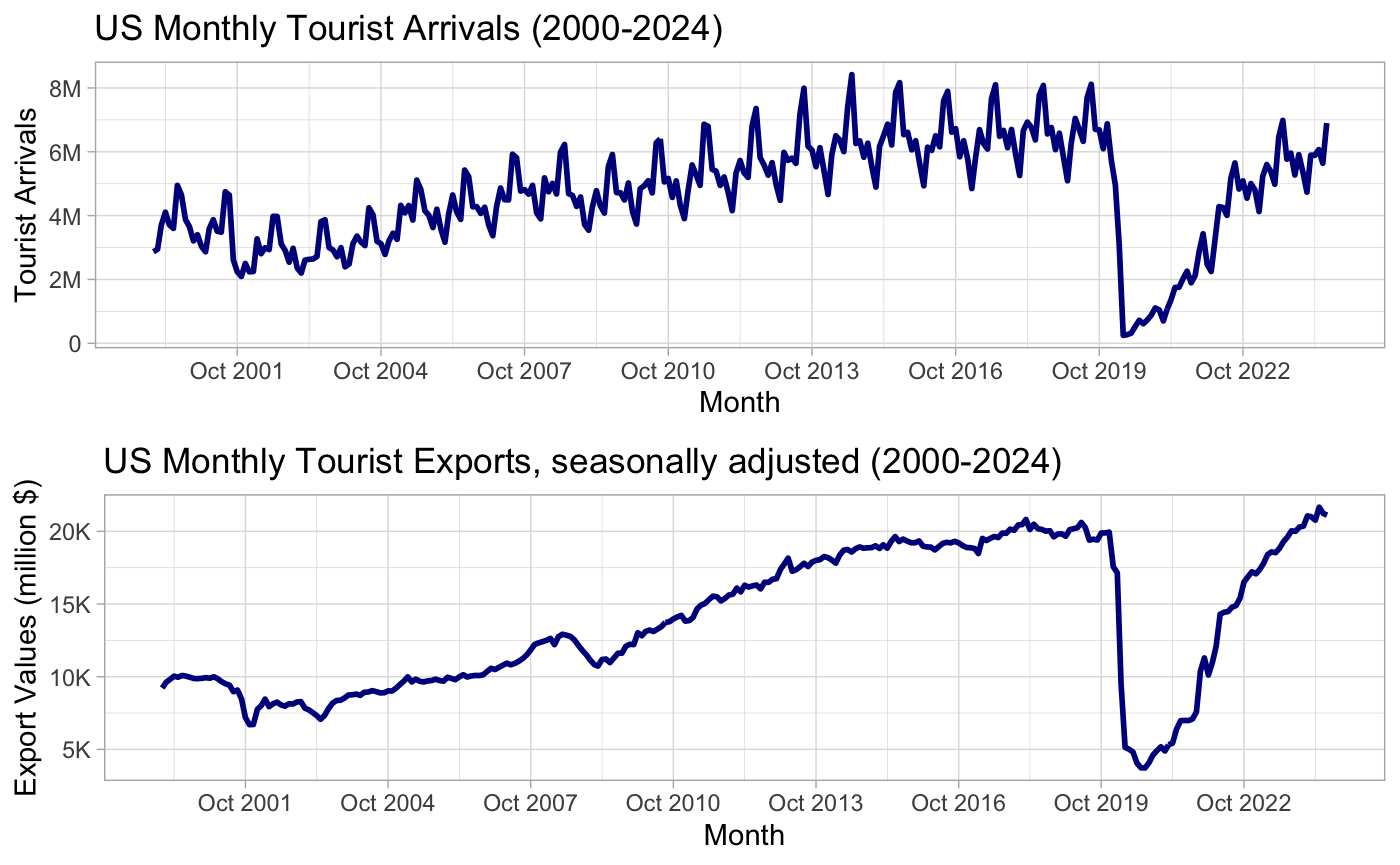
\includegraphics[width=0.85\textwidth]{figures/image2.png}

\textbf{Figure 1.} U.S. monthly tourist arrivals and spending between January 2000 and July 2024.
\end{center}
\bigskip

\begin{center}
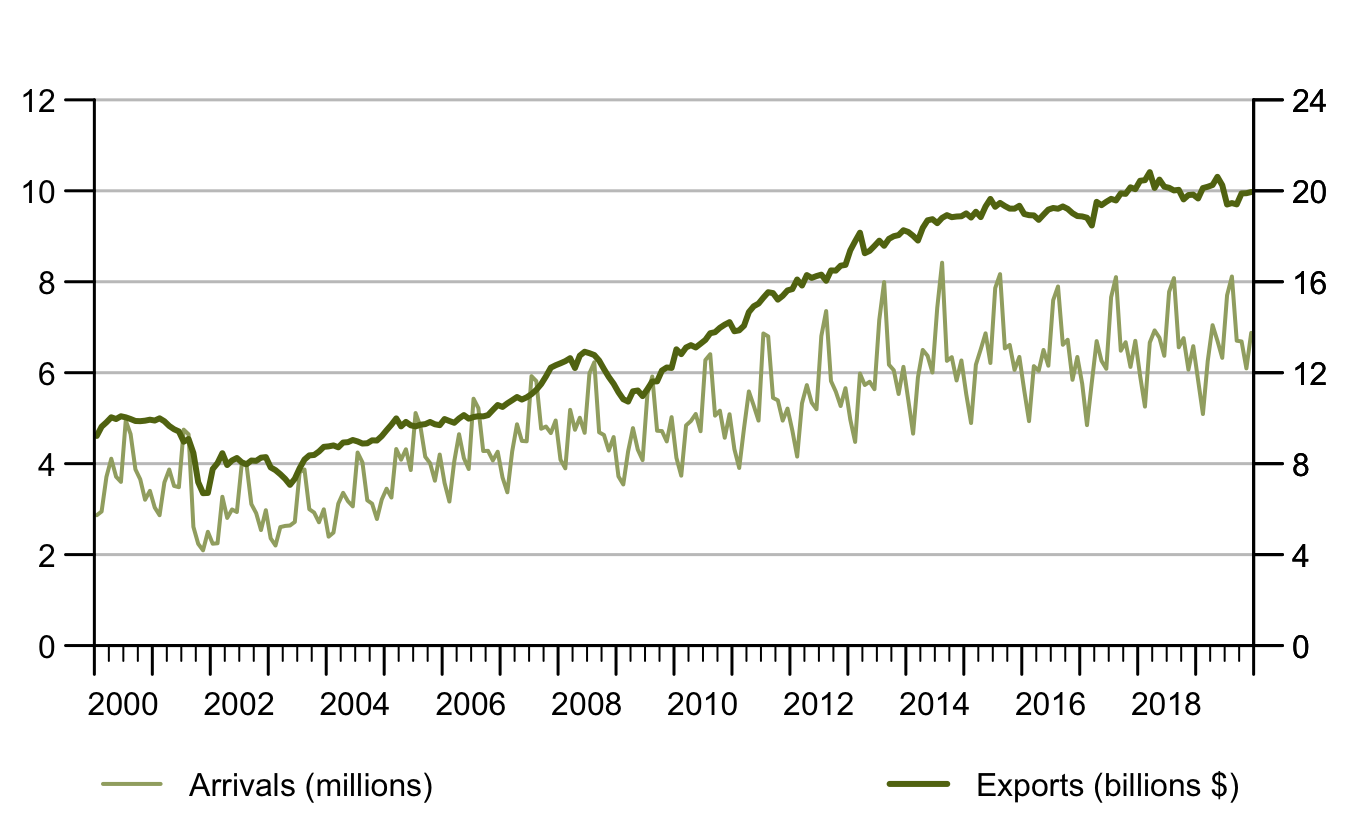
\includegraphics[width=0.8\textwidth]{figures/image3.png}

\textbf{Figure 2.} U.S. monthly tourist arrivals and spending between January 2000 and December 2019. \emph{(Later analyses focus on these time series)}
\end{center}
\bigskip

\begin{center}
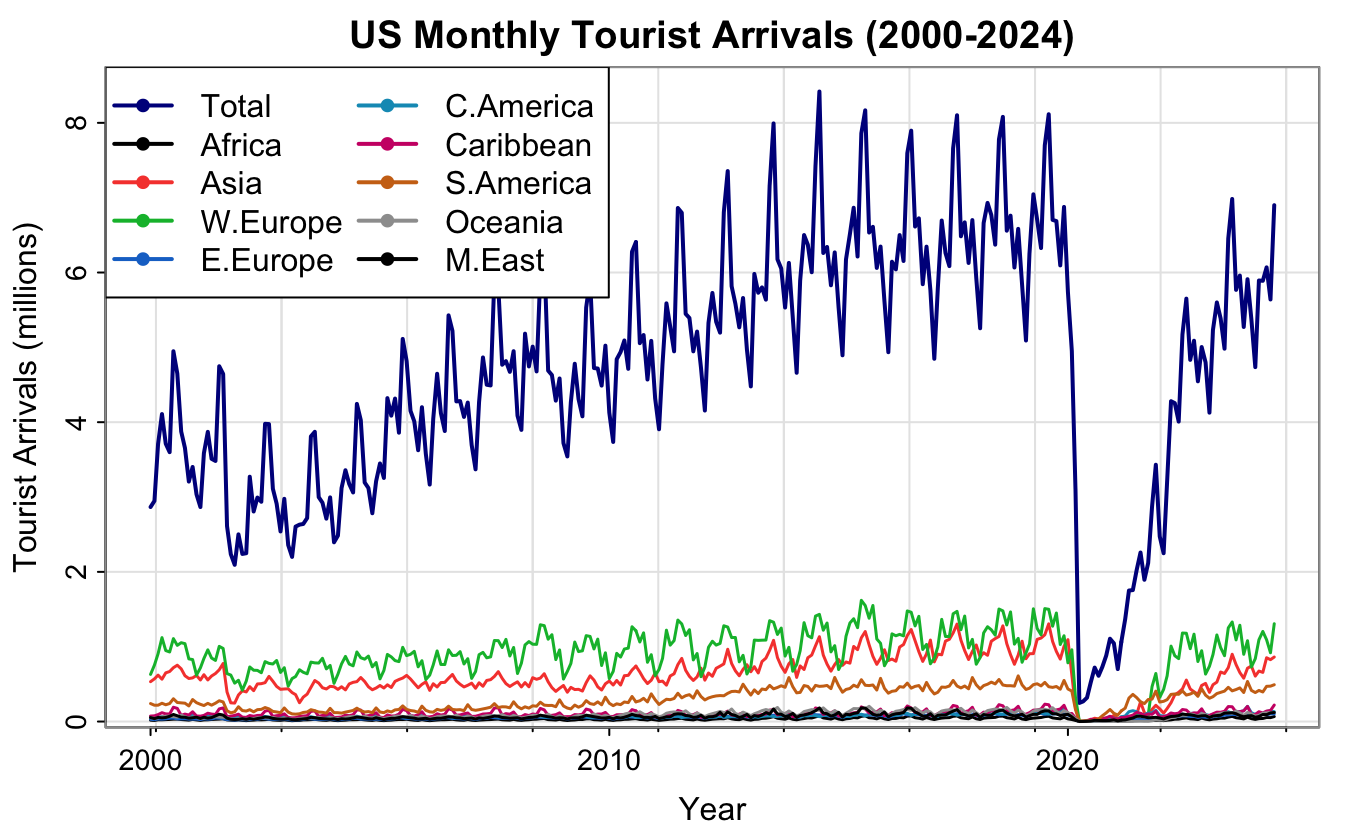
\includegraphics[width=0.85\textwidth]{figures/image4.png}

\textbf{Figure 3.} U.S. monthly tourist arrivals by regions of residence between January 2000 and July 2024. \emph{(Later analysis excludes data since 2020)}
\end{center}
\bigskip

\begin{center}
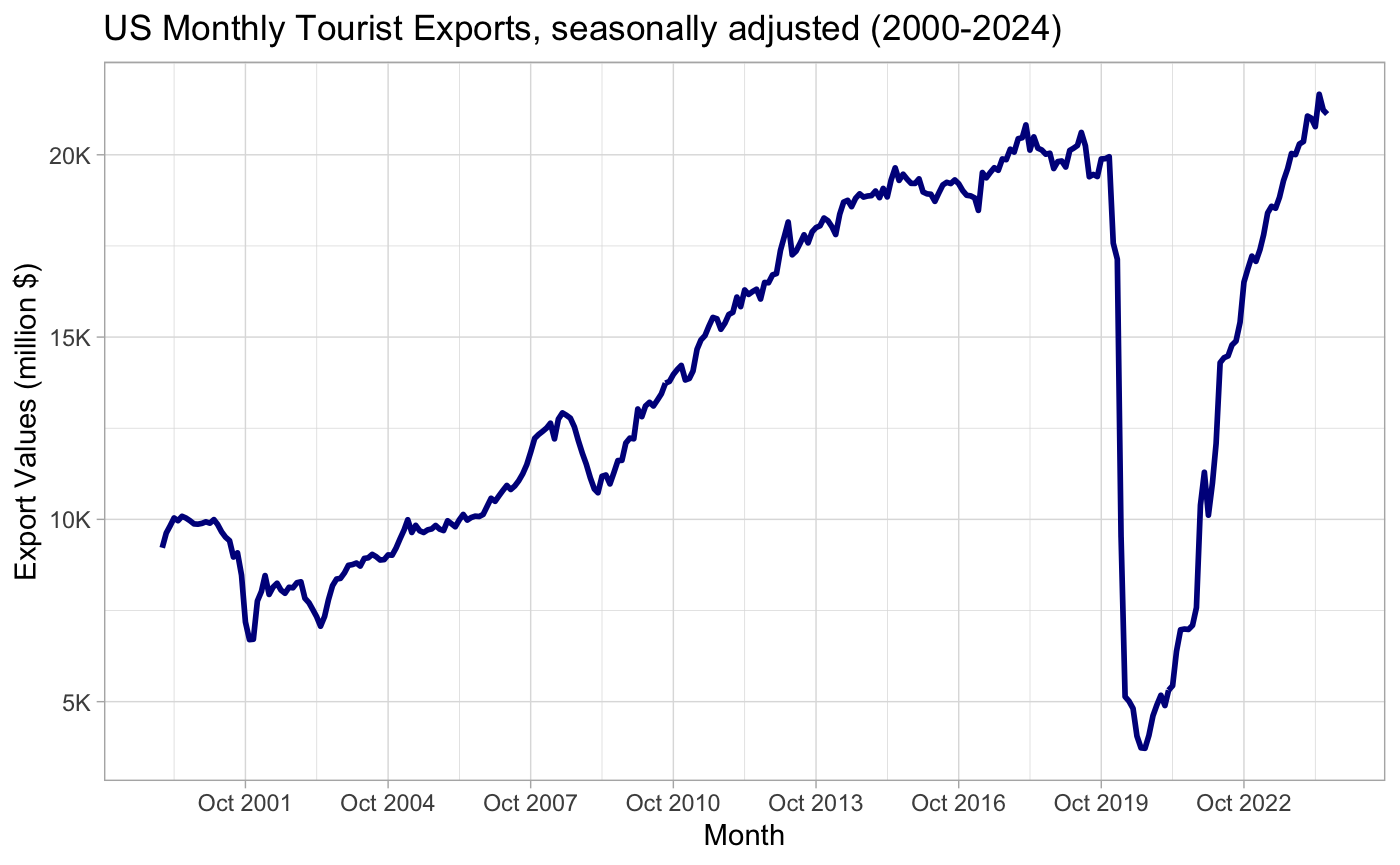
\includegraphics[width=0.85\textwidth]{figures/image5.png}

\textbf{Figure 4.} U.S. monthly tourist spending between January 2000 and July 2024. \emph{(Later analysis excludes data since 2020)}
\end{center}
\bigskip

\begin{center}
\begin{minipage}{0.48\textwidth}\centering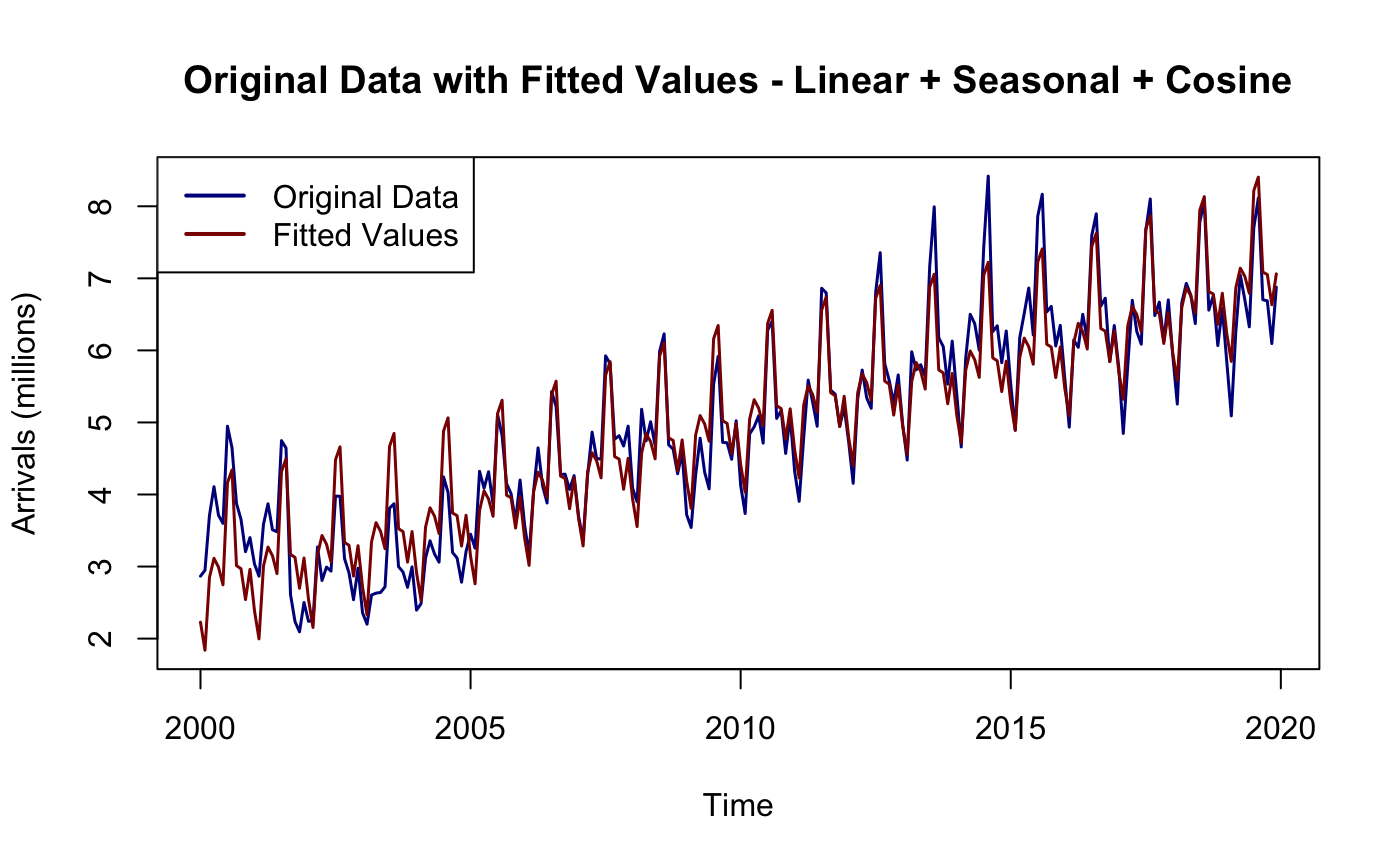
\includegraphics[width=\textwidth]{figures/image6.png}\end{minipage}
\begin{minipage}{0.48\textwidth}\centering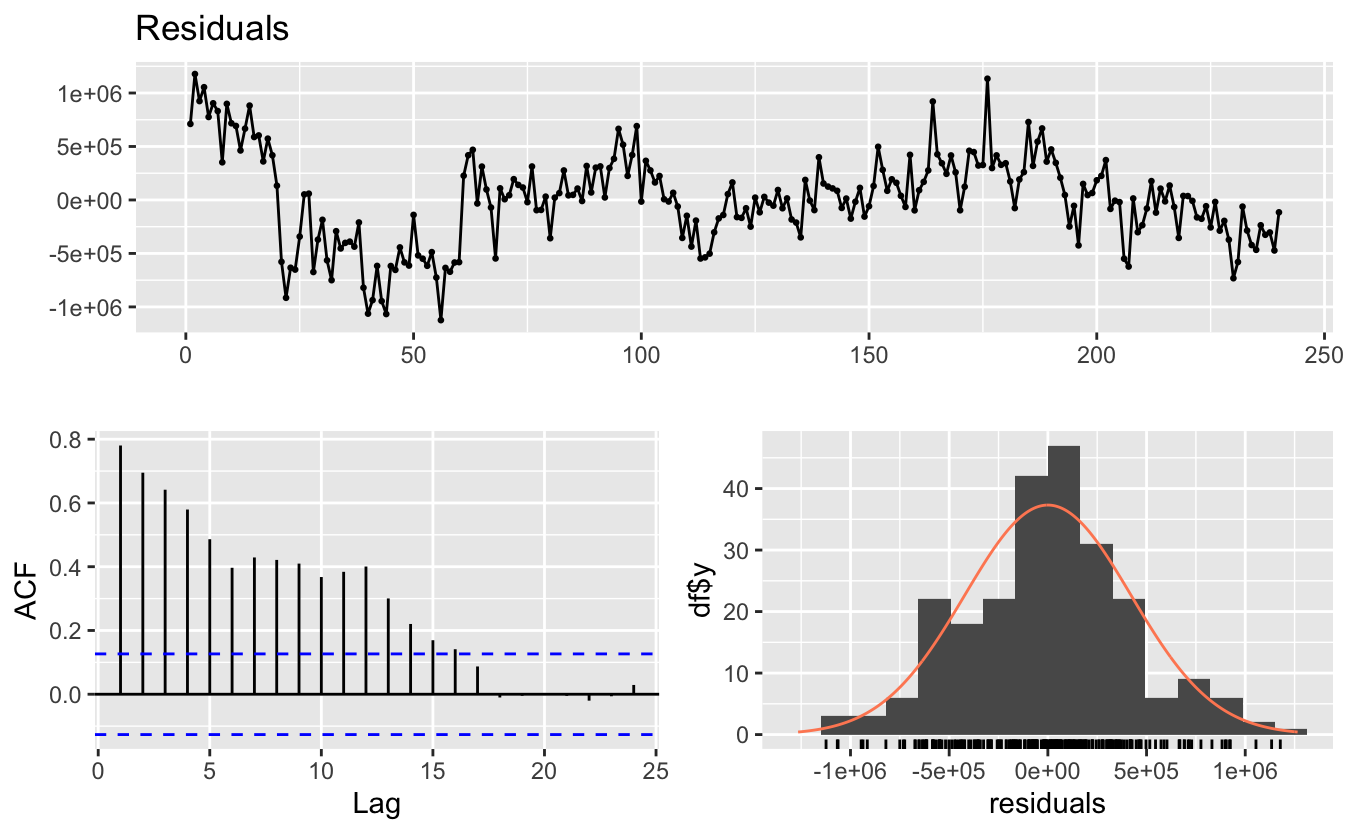
\includegraphics[width=\textwidth]{figures/image7.png}\end{minipage}\\[0.5em]
\begin{minipage}{0.48\textwidth}\centering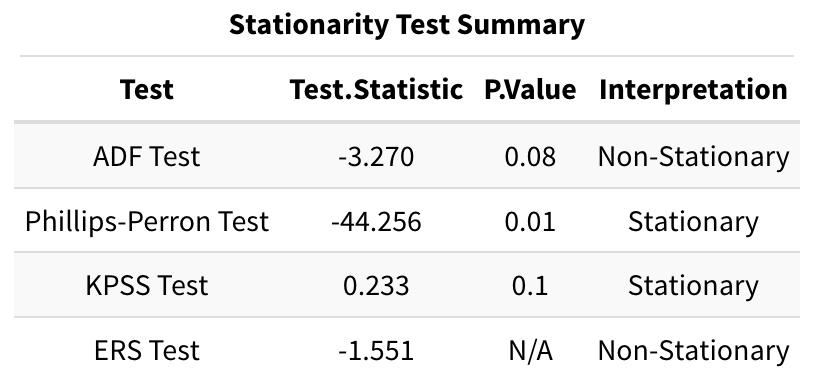
\includegraphics[width=\textwidth]{figures/image8.png}\end{minipage}
\begin{minipage}{0.48\textwidth}\centering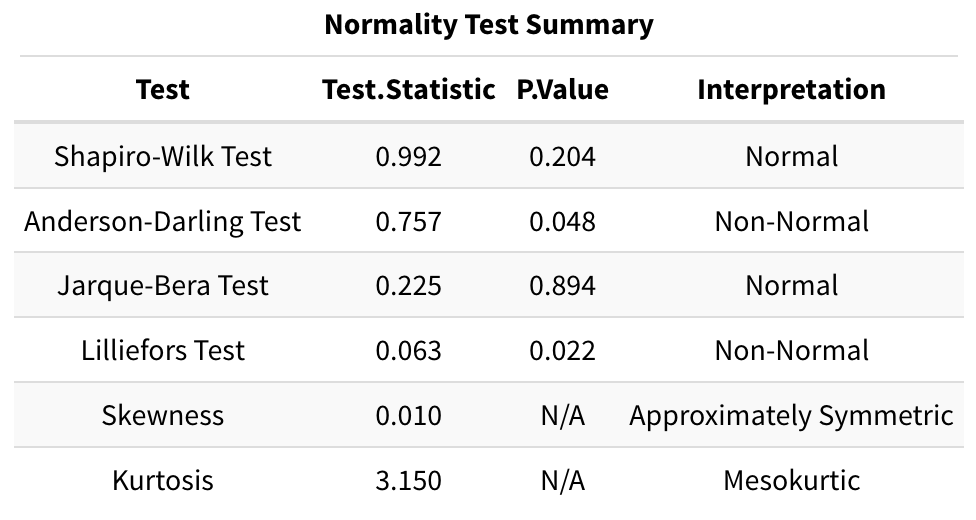
\includegraphics[width=\textwidth]{figures/image9.png}\end{minipage}

\textbf{Figure 5.} Linear + Seasonal + Cosine model fitted to monthly tourist arrivals data. The model's residuals are not independent, not stationary, and not normal, suggesting poor reliability of forecasts.
\end{center}
\bigskip

\begin{center}
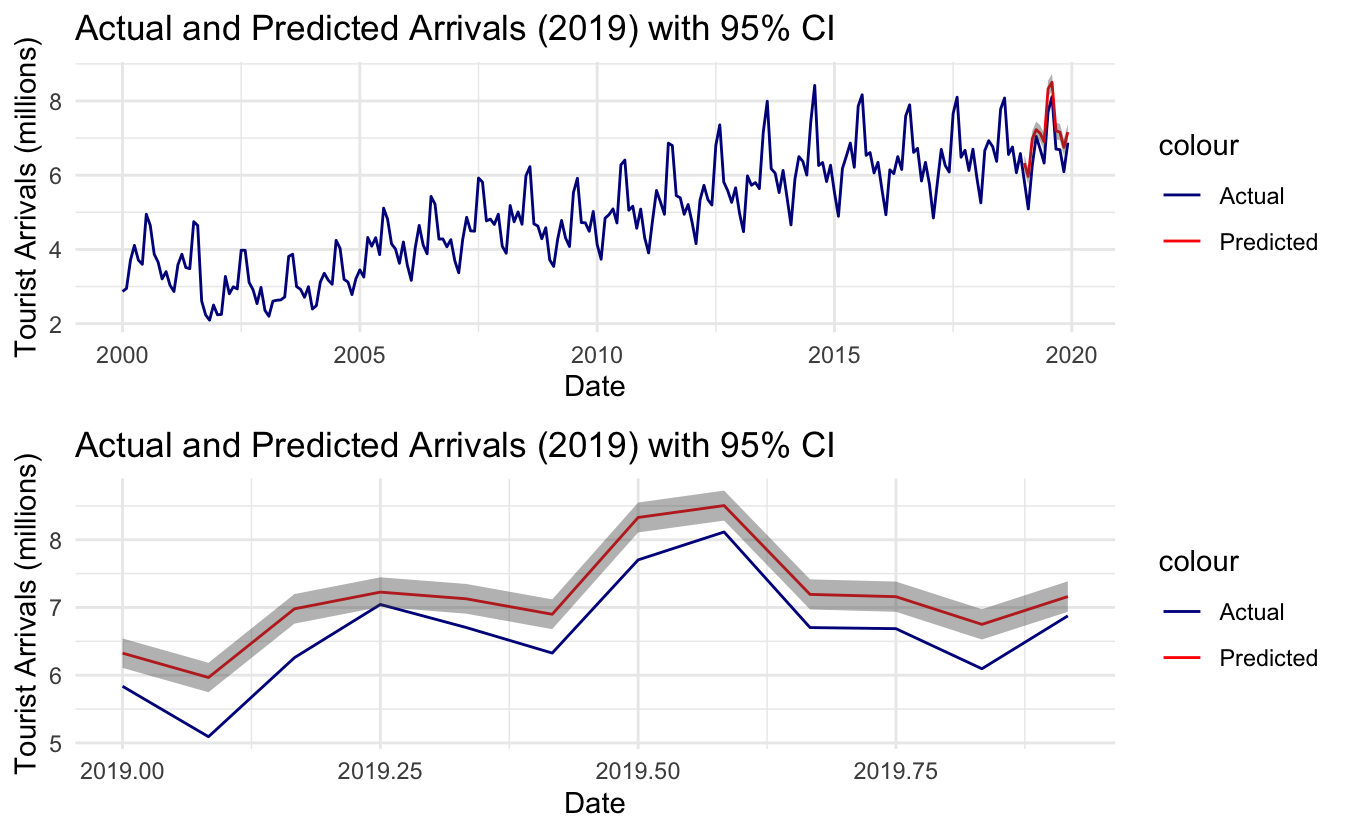
\includegraphics[width=0.85\textwidth]{figures/image10.png}

\textbf{Figure 6.} Cross-validation of Linear + Seasonal + Cosine model for US monthly tourist arrivals, trained on data up to 2018 and tested on actual data from 2019.
\end{center}
\bigskip

\begin{center}
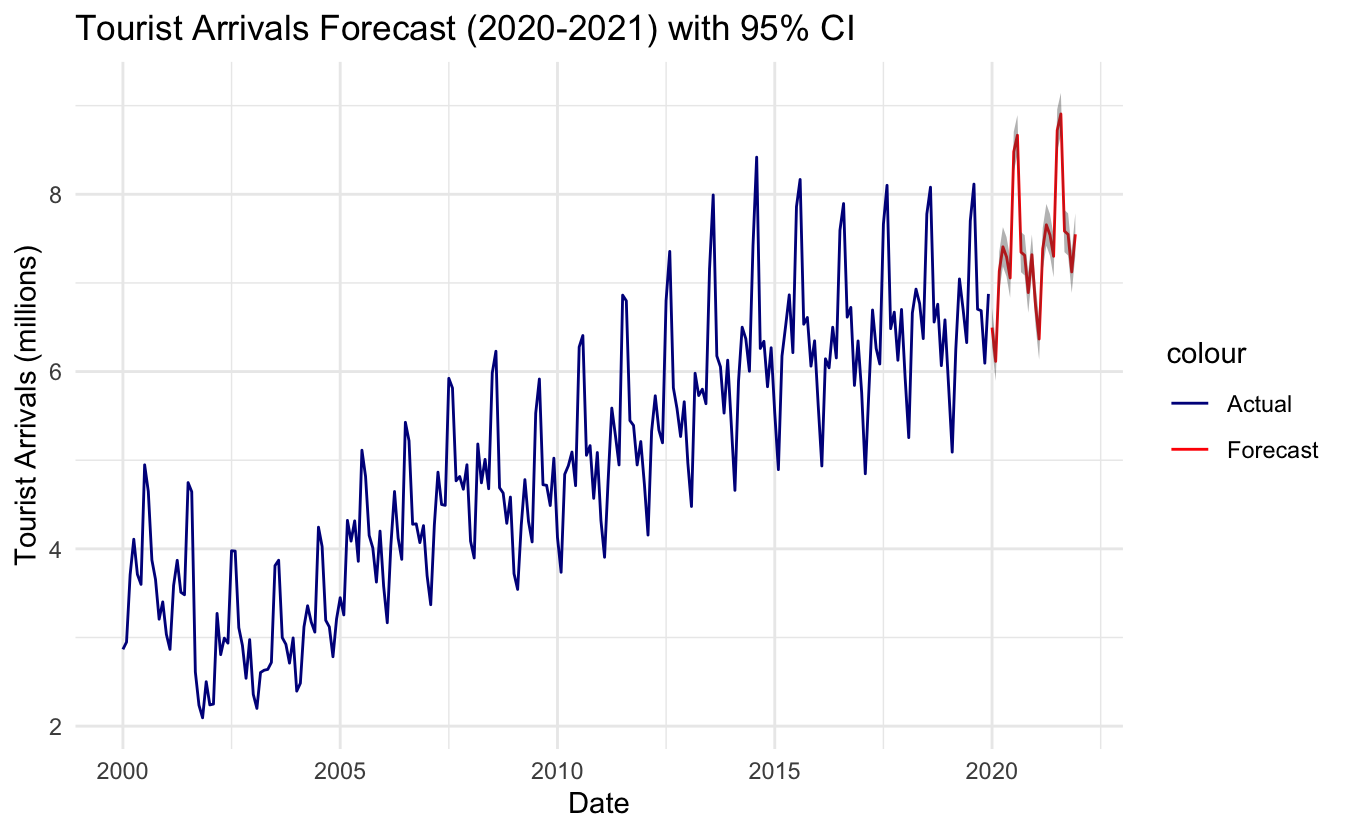
\includegraphics[width=0.85\textwidth]{figures/image11.png}

\textbf{Figure 7.} Predictions for hypothetical 2020 and 2021 data (without COVID-19 pandemic), based on the Linear + Seasonal + Cosine model for US monthly arrivals.
\end{center}
\bigskip

\begin{center}
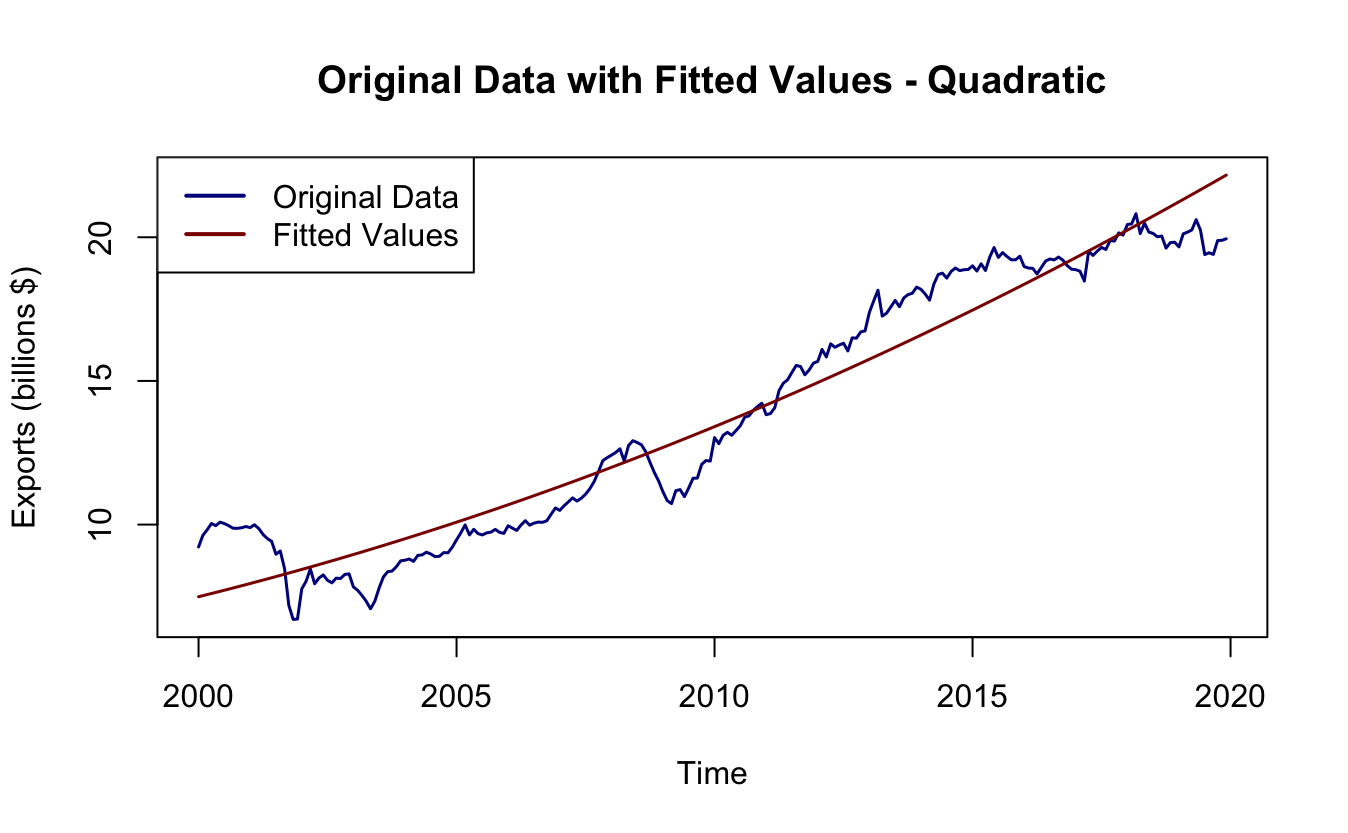
\includegraphics[width=0.7\textwidth]{figures/image12.png}\\[0.5em]
\begin{minipage}{0.32\textwidth}\centering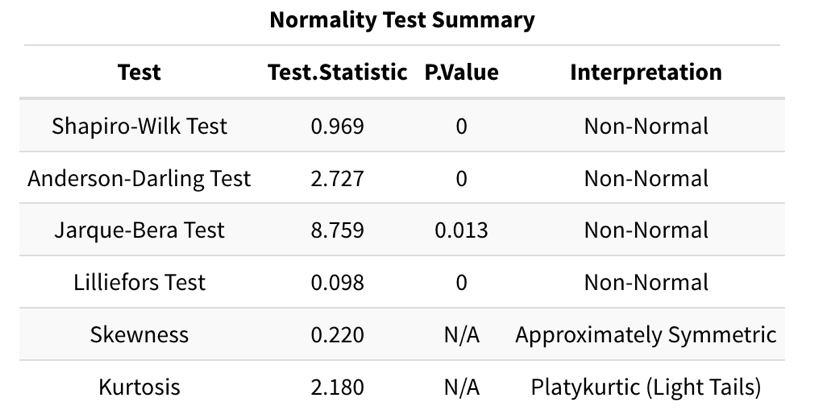
\includegraphics[width=\textwidth]{figures/image13.png}\end{minipage}
\begin{minipage}{0.32\textwidth}\centering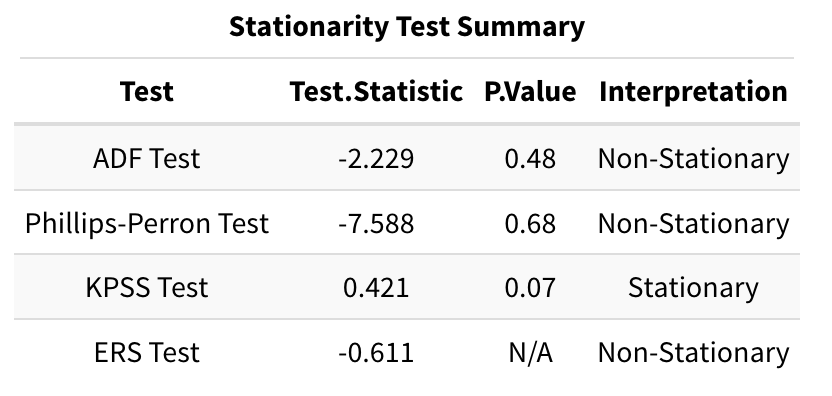
\includegraphics[width=\textwidth]{figures/image14.png}\end{minipage}
\begin{minipage}{0.32\textwidth}\centering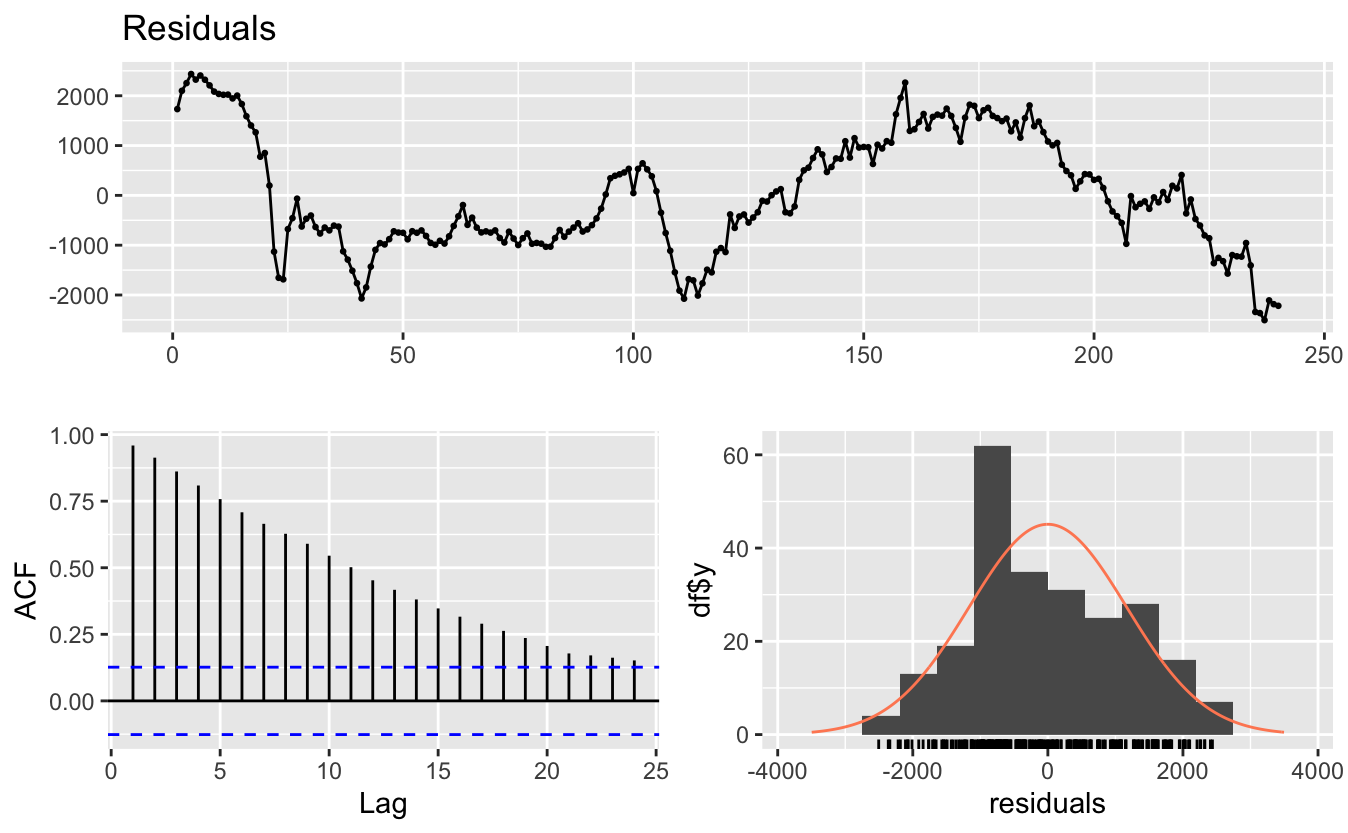
\includegraphics[width=\textwidth]{figures/image15.png}\end{minipage}

\textbf{Figure 8.} Quadratic model fitted to monthly tourist exports data. The model's residuals are not independent, not stationary, and not normal, suggesting poor reliability of forecasts.
\end{center}
\bigskip

\begin{center}
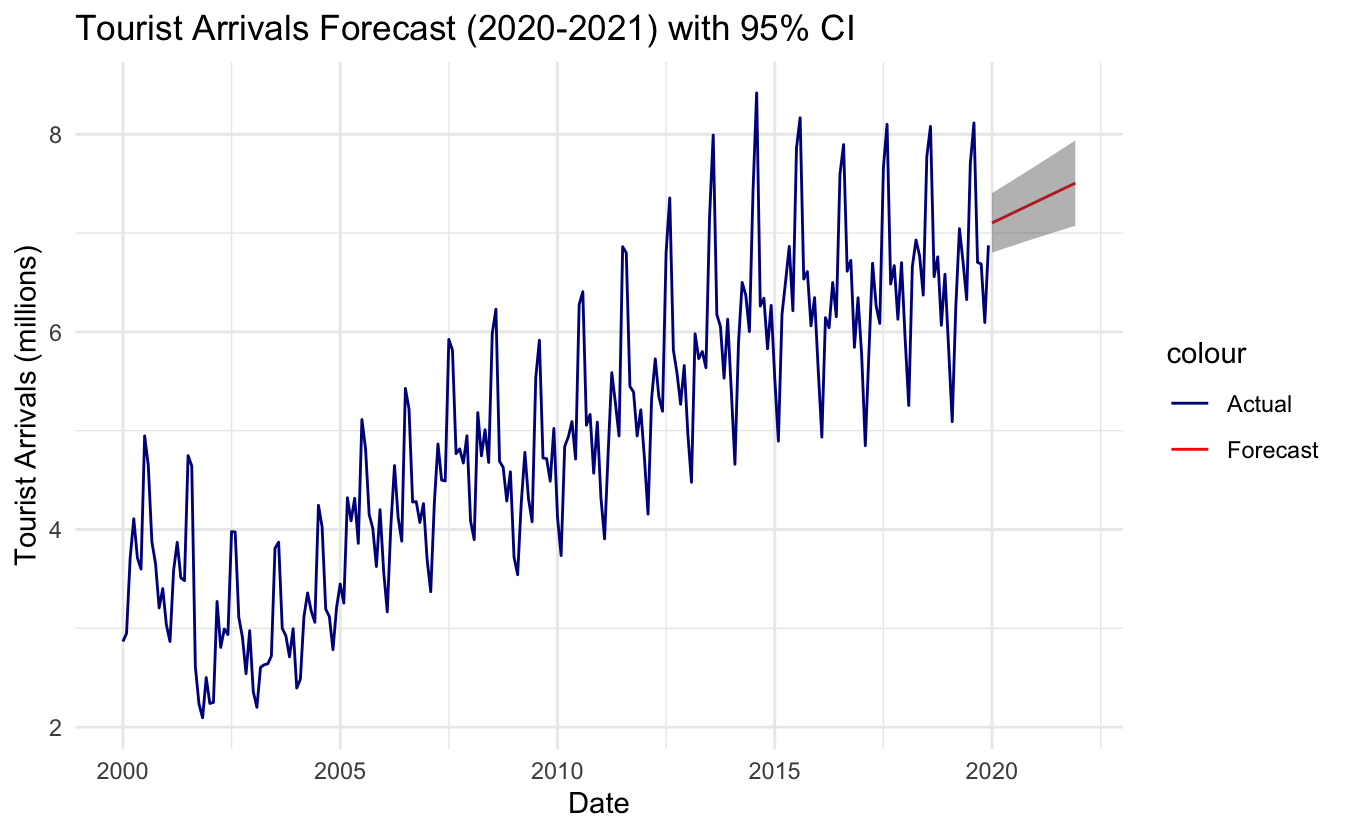
\includegraphics[width=0.9\textwidth]{figures/image16.png}

\textbf{Figure 9.} Predictions for hypothetical 2020 and 2021 data (without COVID-19 pandemic), based on the Quadratic model for US monthly tourist exports.
\end{center}
\bigskip

\begin{center}
\begin{minipage}{0.48\textwidth}\centering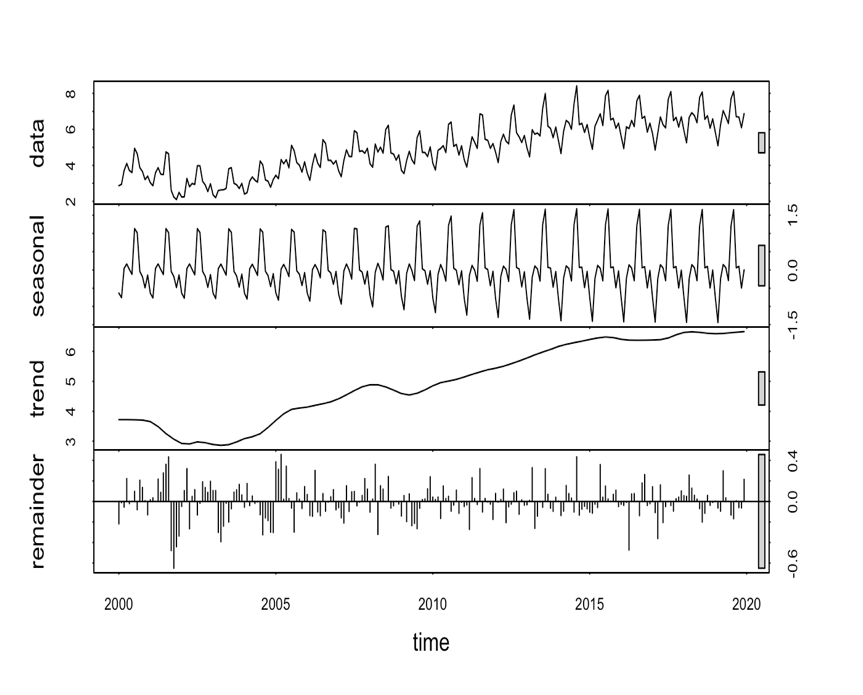
\includegraphics[width=\textwidth]{figures/image17.png}\\ a. Tourist Arrivals\end{minipage}
\begin{minipage}{0.48\textwidth}\centering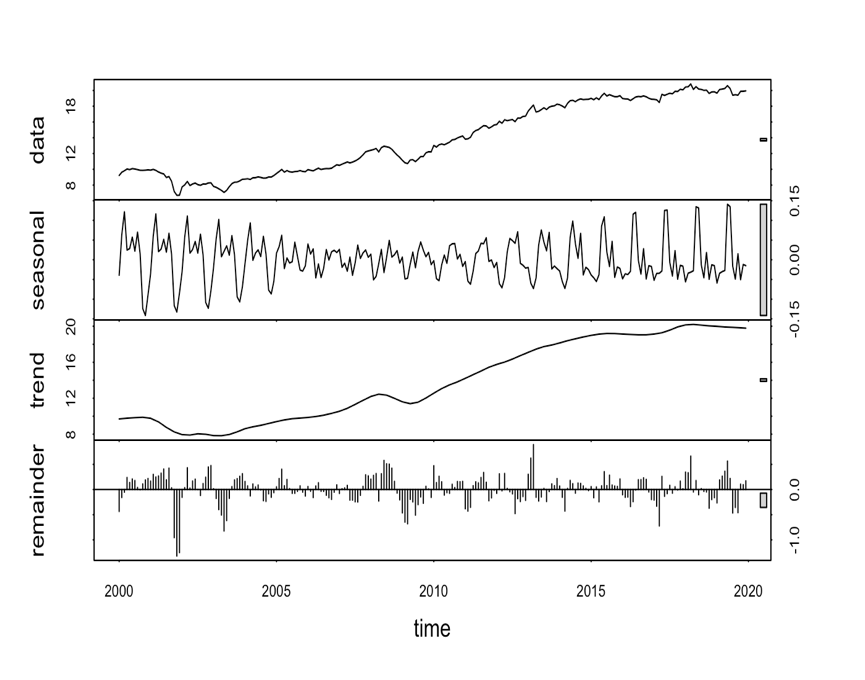
\includegraphics[width=\textwidth]{figures/image18.png}\\ b. Tourist Spending\end{minipage}

\textbf{Figure 10.} STL decomposition of US monthly tourist arrivals and spending between 2000 and 2019.
\end{center}
\bigskip

\begin{center}
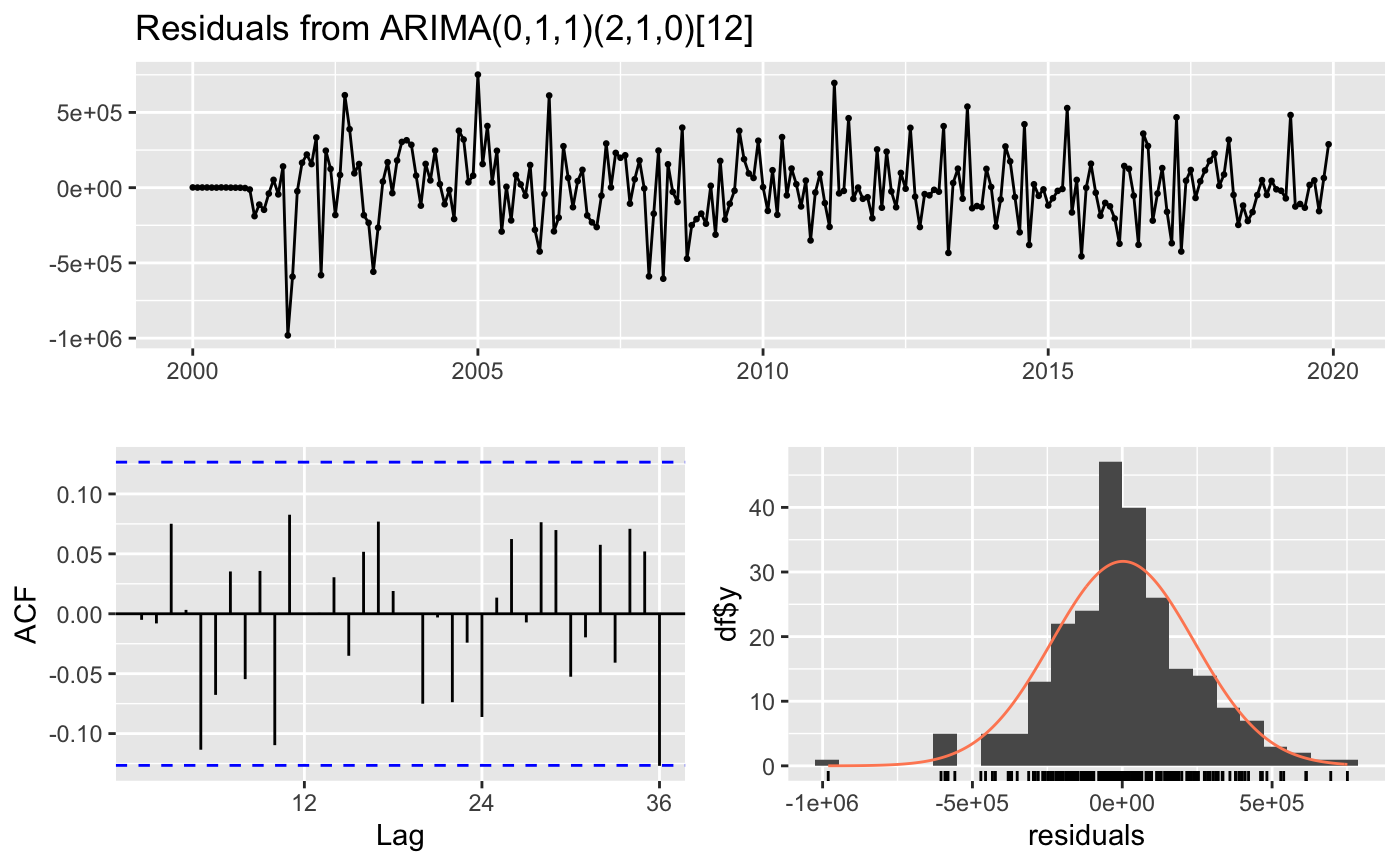
\includegraphics[width=0.85\textwidth]{figures/image19.png}\\[0.5em]
\begin{minipage}{0.48\textwidth}\centering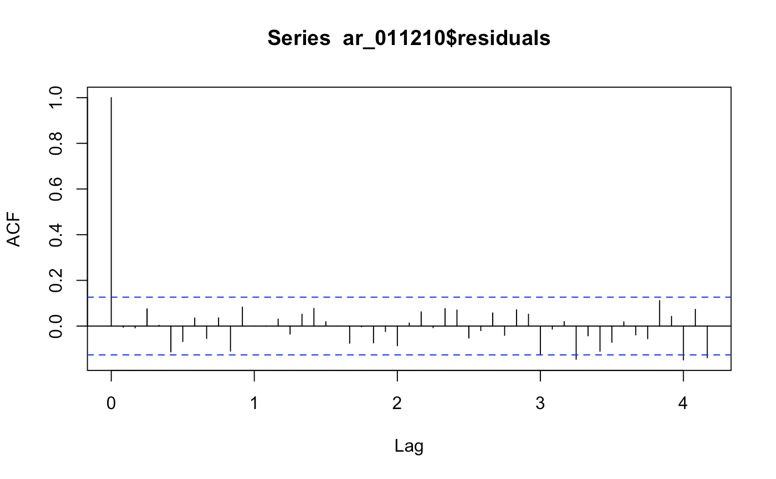
\includegraphics[width=\textwidth]{figures/image20.png}\end{minipage}
\begin{minipage}{0.48\textwidth}\centering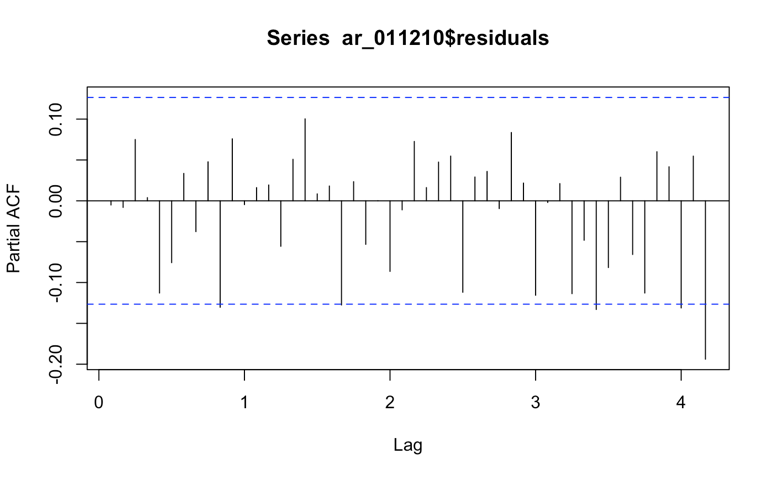
\includegraphics[width=\textwidth]{figures/image21.png}\end{minipage}\\[0.5em]
\begin{minipage}{0.48\textwidth}\centering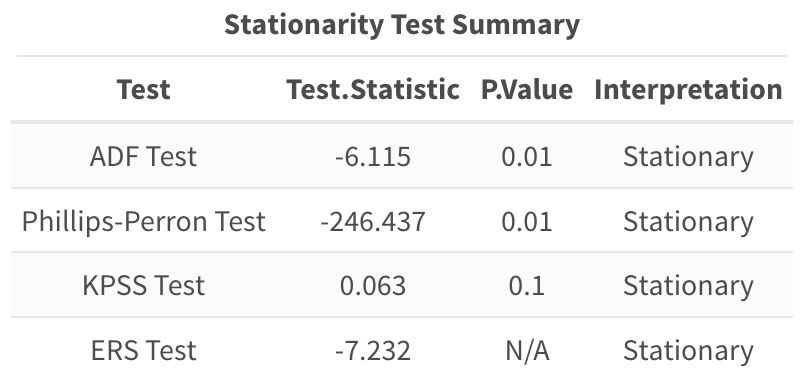
\includegraphics[width=\textwidth]{figures/image22.png}\end{minipage}
\begin{minipage}{0.48\textwidth}\centering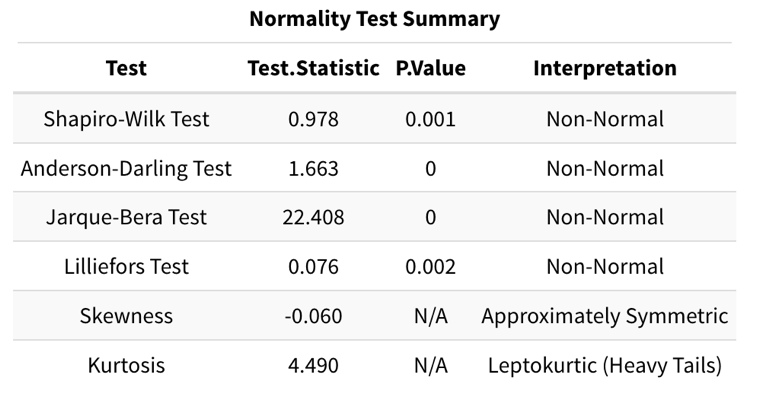
\includegraphics[width=\textwidth]{figures/image23.png}\end{minipage}

\textbf{Figure 11.} $ARIMA(0,1,1)\times(2,1,0)_{12}$ fitted on US monthly tourist arrivals data. The model's residuals are independent, stationary, but not normal, suggesting interpreting forecasts with caution.
\end{center}
\bigskip

\begin{center}
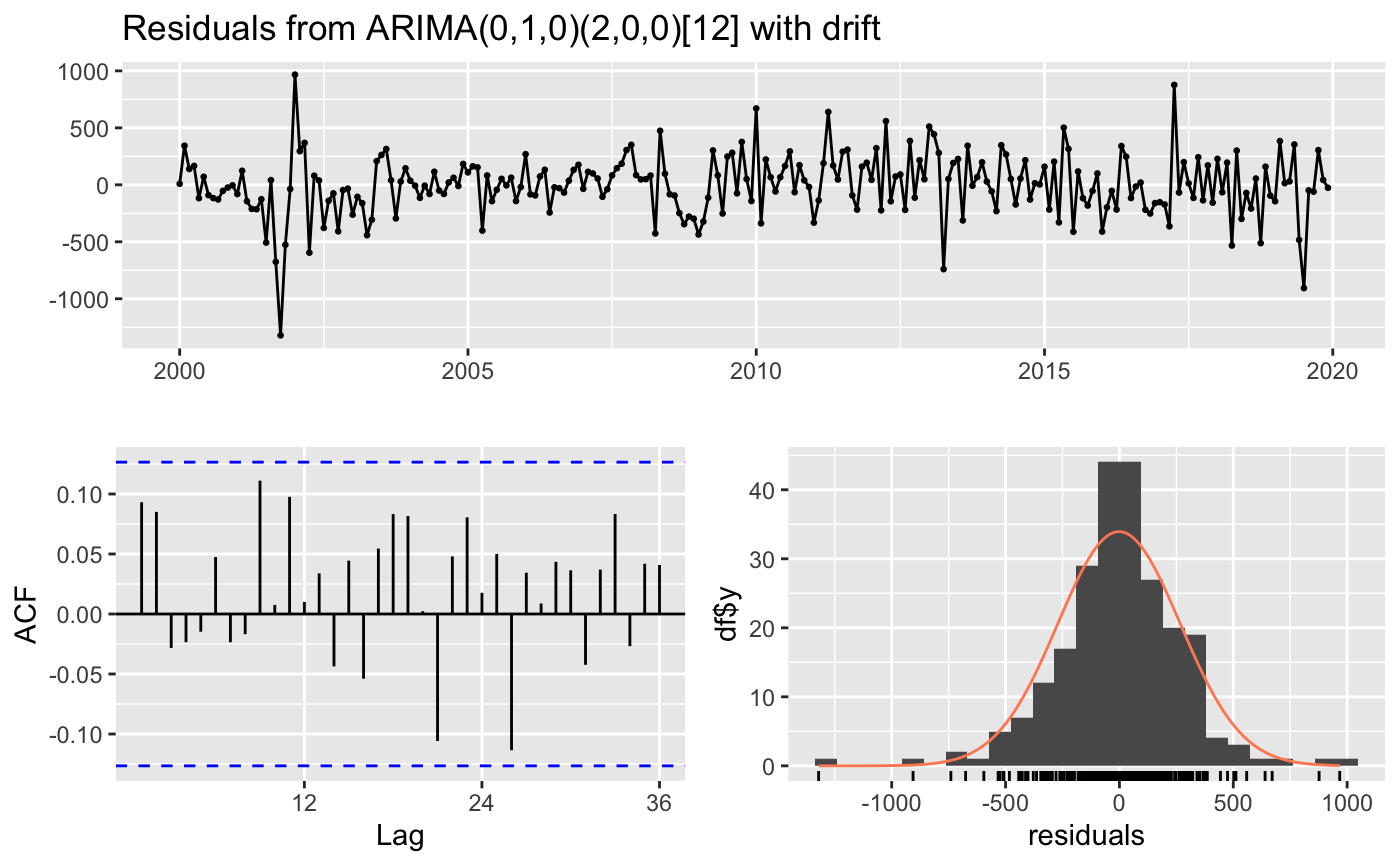
\includegraphics[width=0.85\textwidth]{figures/image24.png}\\[0.5em]
\begin{minipage}{0.48\textwidth}\centering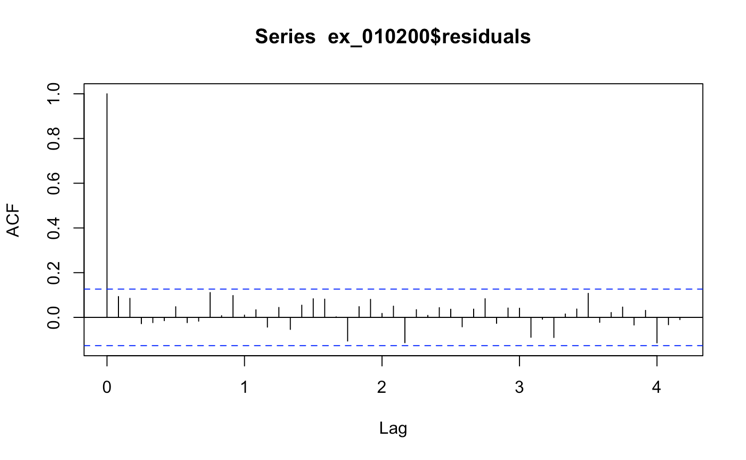
\includegraphics[width=\textwidth]{figures/image25.png}\end{minipage}
\begin{minipage}{0.48\textwidth}\centering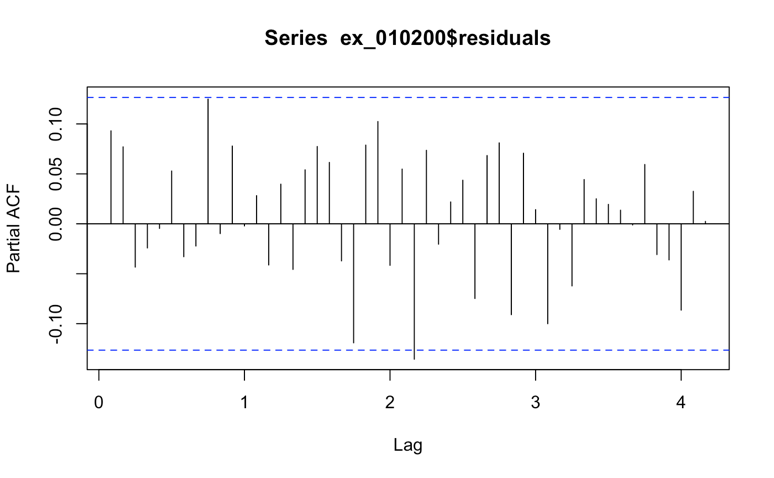
\includegraphics[width=\textwidth]{figures/image26.png}\end{minipage}\\[0.5em]
\begin{minipage}{0.48\textwidth}\centering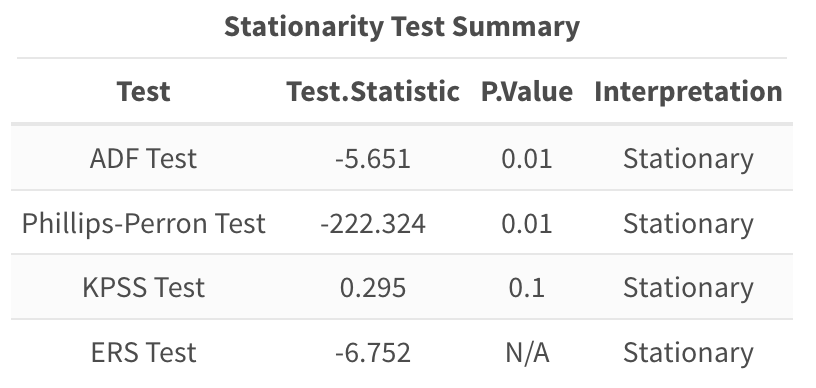
\includegraphics[width=\textwidth]{figures/image27.png}\end{minipage}
\begin{minipage}{0.48\textwidth}\centering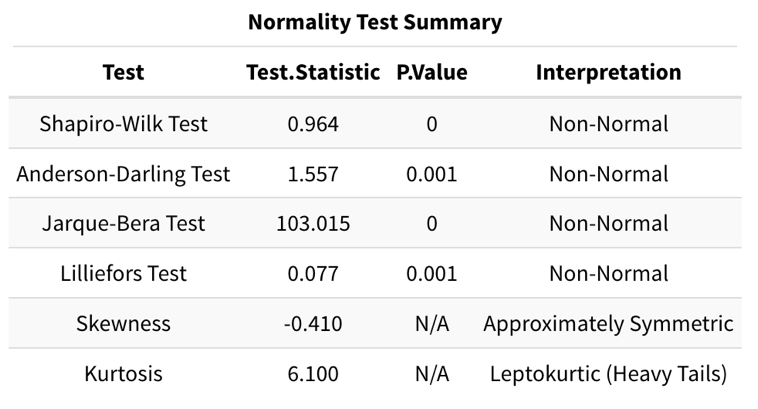
\includegraphics[width=\textwidth]{figures/image28.png}\end{minipage}

\textbf{Figure 12.} $ARIMA(0,1,0)\times(2,0,0)_{12}$ fitted on US monthly tourist exports data. The model's residuals are independent, stationary, but not normal, suggesting interpreting forecasts with caution.
\end{center}
\bigskip

\begin{center}
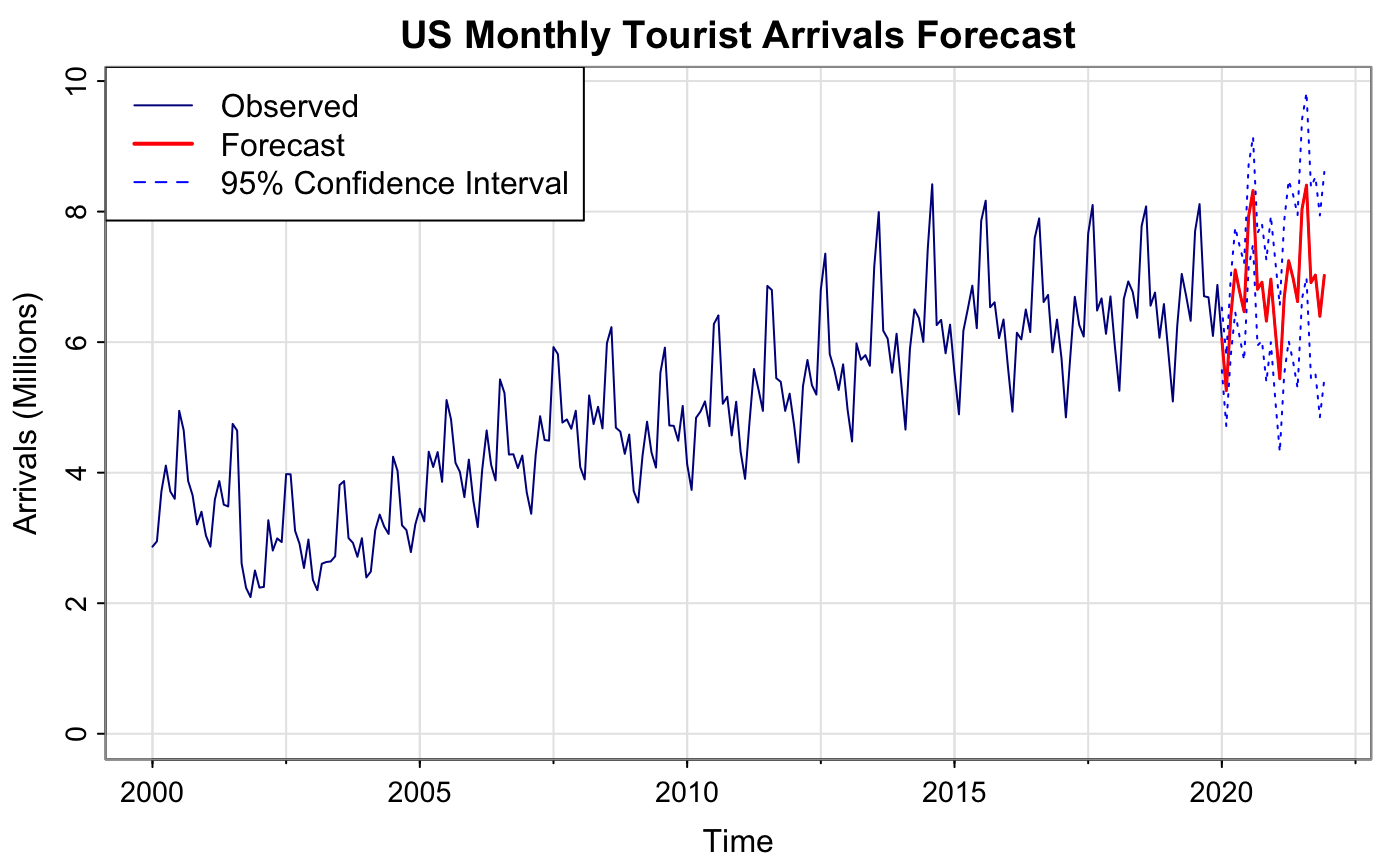
\includegraphics[width=0.85\textwidth]{figures/image29.png}

\textbf{Figure 13.} Forecasts for monthly arrivals in 2020 and 2021, assuming the absence of COVID-19 pandemic, based on the $ARIMA(0,1,1)\times(2,1,0)_{12}$ fitted on historical data.
\end{center}
\bigskip

\begin{center}
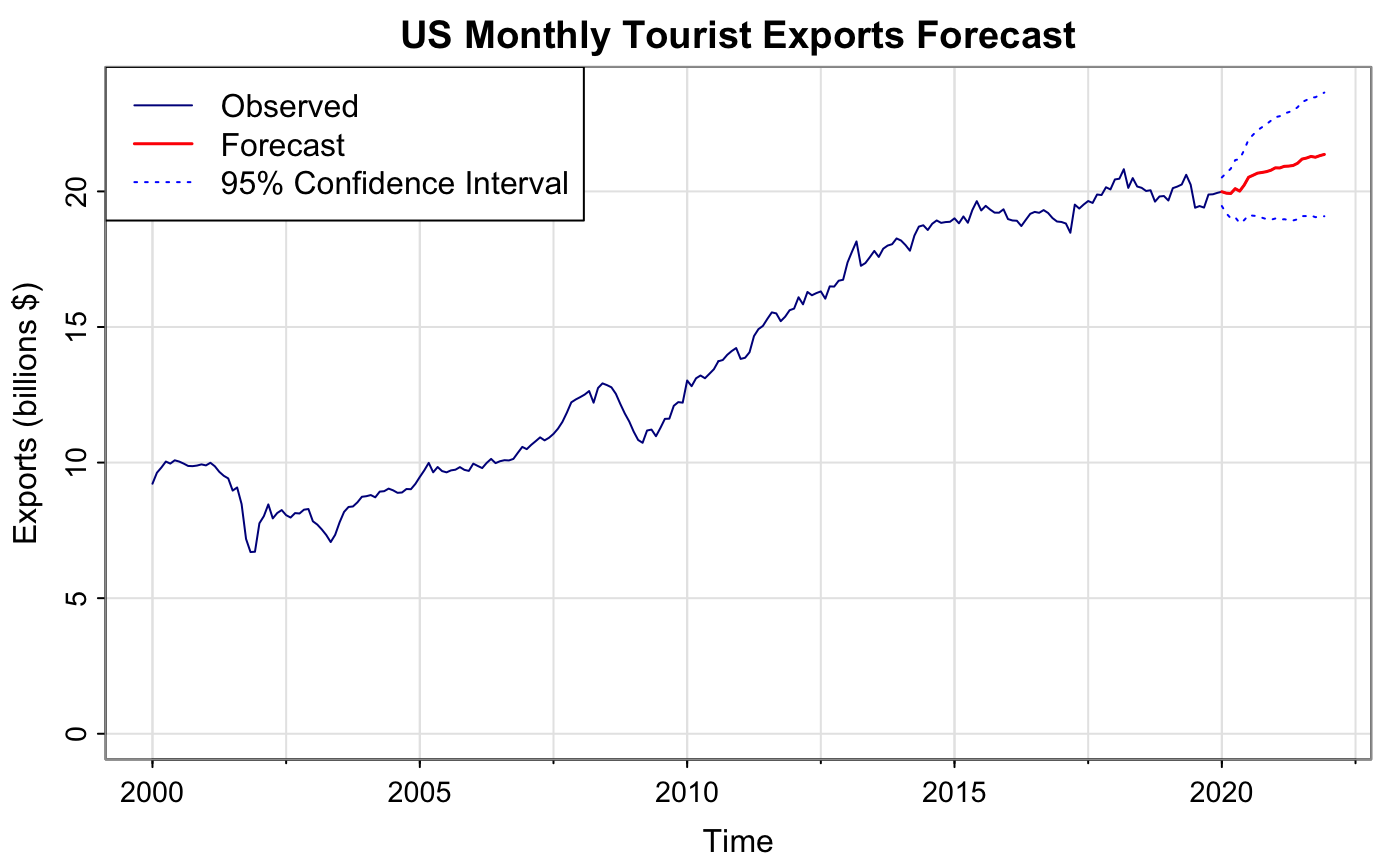
\includegraphics[width=0.9\textwidth]{figures/image30.png}

\textbf{Figure 14.} Forecasts for monthly exports in 2020 and 2021, assuming the absence of COVID-19 pandemic, based on the $ARIMA(0,1,0)\times(2,0,0)_{12}$ fitted on historical data.
\end{center}
\bigskip

\subsection{Summary Tables}

\begin{center}
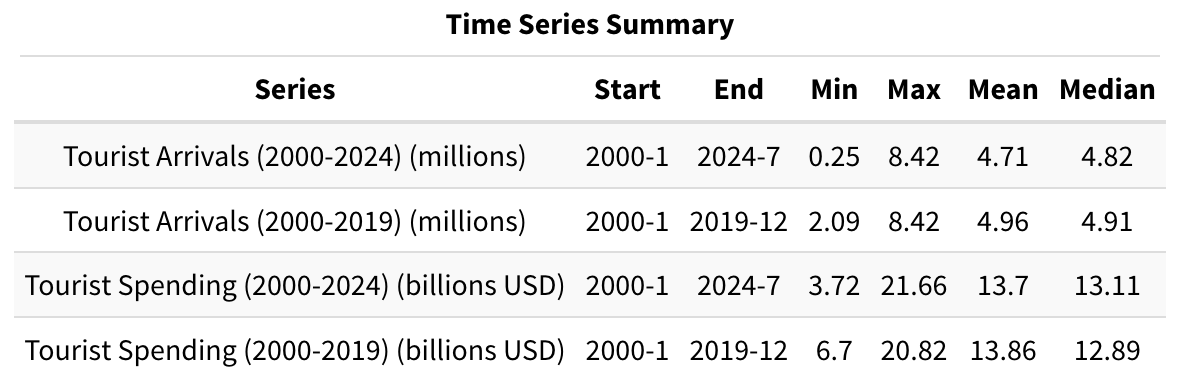
\includegraphics[width=1\textwidth]{figures/image31.png}

\textbf{Table 1.} Key statistics of working time series
\end{center}
\bigskip

\begin{center}
\begin{minipage}{0.48\textwidth}\centering
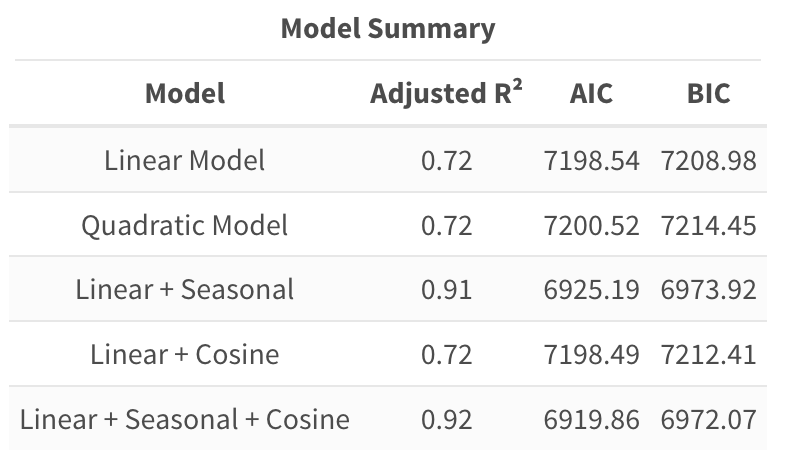
\includegraphics[width=\textwidth]{figures/image32.png}\\[0.3em]
\textbf{Table 2.} Comparisons of time models on monthly tourist arrivals
\end{minipage}
\begin{minipage}{0.48\textwidth}\centering
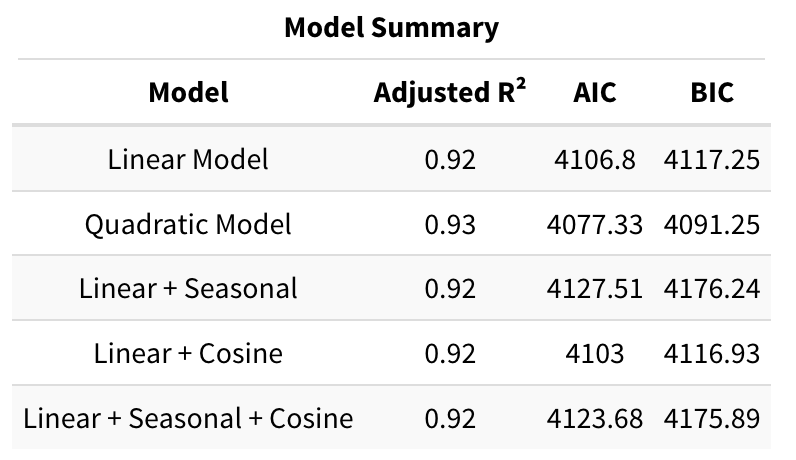
\includegraphics[width=\textwidth]{figures/image33.png}\\[0.3em]
\textbf{Table 3.} Comparisons of time models on monthly tourist exports
\end{minipage}\\[1em]
\begin{minipage}{0.48\textwidth}\centering
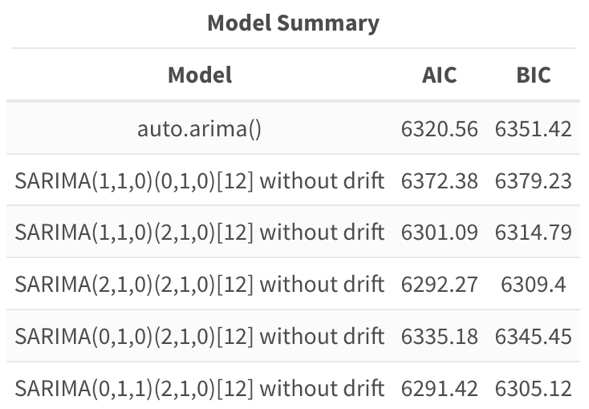
\includegraphics[width=\textwidth]{figures/image34.png}\\[0.3em]
\textbf{Table 4.} Comparisons of SARIMA models on monthly tourist arrivals
\end{minipage}
\begin{minipage}{0.48\textwidth}\centering
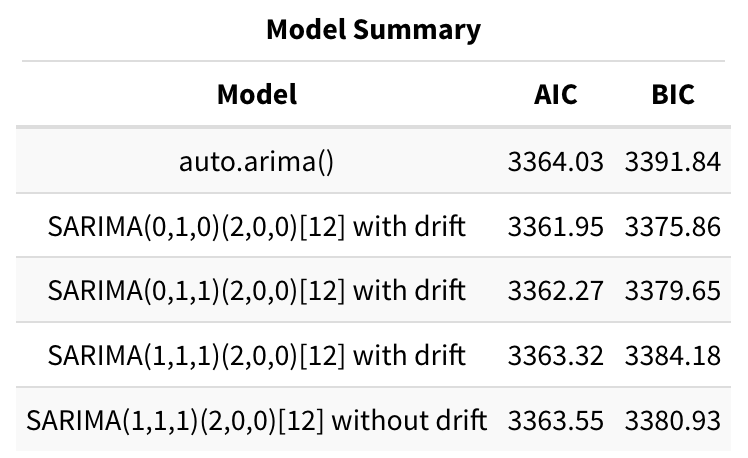
\includegraphics[width=\textwidth]{figures/image35.png}\\[0.3em]
\textbf{Table 5.} Comparisons of SARIMA models on monthly tourist exports
\end{minipage}
\end{center}
\bigskip

\begin{center}
\textbf{Table 6.} Equations for SARIMA models.
\smallskip

\begin{tabular}{@{}p{0.32\textwidth} p{0.58\textwidth}@{}}
\toprule
\textbf{Time Series} & \textbf{Best Fitting SARIMA Equations} \\
\midrule
Monthly Tourist Arrivals \newline $(0,1,1)\times(2,1,0)_{12}$ & $\nabla_{12}\nabla A_{t} = -0.4713\,\epsilon_{t-1} - 0.6017\,A_{t-12} - 0.3783\,A_{t-24} + \epsilon_{t}$ \\[0.8em]
Monthly Tourist Exports \newline $(0,1,0)\times(2,0,0)_{12}$ & $\nabla X_{t} = -0.2526\,X_{t-12} - 0.1882\,X_{t-24} + 47.2346 + \epsilon_{t}$ \newline Or: \newline $X_{t} = X_{t-1} - 0.2526\,X_{t-12} - 0.1882\,X_{t-24} + 47.2346 + \epsilon_{t}$ \\
\bottomrule
\end{tabular}
\end{center}
\bigskip

\begin{center}
\textbf{Table 7.} Comparison of AIC and BIC values among the best-fitting models.
\smallskip

\begin{tabular}{@{}l l c c@{}}
\toprule
\textbf{Time Series} & \textbf{Model Type} & \textbf{AIC} & \textbf{BIC} \\
\midrule
\multirow{2}{*}{Monthly Tourist Arrivals} & Function of Time & 6919.86 & 6972.07 \\
 & SARIMA & 6291.42 & 6305.12 \\
\multirow{2}{*}{Monthly Tourist Exports} & Function of Time & 4077.33 & 4091.25 \\
 & SARIMA & 3361.95 & 3375.86 \\
\bottomrule
\end{tabular}
\end{center}
\bigskip

\subsection{Statistical Tests \& Methods}

Below is a brief introduction to each statistical test and method utilized in this analysis. Sources of information that helped in compiling these summaries are listed in the References section.

\paragraph{ADF (Augmented Dickey-Fuller) Test}

The ADF test checks if a time series is stationary by testing for a unit root. The null hypothesis ($\mathbf{H}_{\mathbf{0}}$) is that the series has a unit root (non-stationary), while the alternative hypothesis ($\mathbf{H}_{\mathbf{1}}$) is that the series is stationary. A significant p-value (typically $<$ 0.05) leads to rejecting $\mathbf{H}_{\mathbf{0}}$, indicating that the series is likely stationary.

\paragraph{Phillips-Perron (PP) Test}

Like the ADF test, the PP test evaluates whether a time series is stationary, accounting for potential serial correlation and heteroskedasticity in errors. Here, $\mathbf{H}_{\mathbf{0}}$ states that the series has a unit root (non-stationary), while rejecting $\mathbf{H}_{\mathbf{0}}$ indicates stationarity. A significant result supports stationarity.

\paragraph{KPSS (Kwiatkowski-Phillips-Schmidt-Shin) Test}

The KPSS test approaches stationarity testing differently, assuming the series is stationary under $\mathbf{H}_{\mathbf{0}}$. If the p-value is small, $\mathbf{H}_{\mathbf{0}}$ is rejected, suggesting the series is non-stationary. This complements ADF and PP tests by testing stationarity as the null.

\paragraph{ERS (Elliott-Rothenberg-Stock) Test}

The ERS test also assesses unit roots, particularly when seeking stationarity in the presence of trend and constant terms. $\mathbf{H}_{\mathbf{0}}$ states the series has a unit root (non-stationary), and rejecting $\mathbf{H}_{\mathbf{0}}$ suggests stationarity. This test is often more sensitive than the ADF test.

\paragraph{ACF (Autocorrelation Function)}

The ACF measures the correlation of a series with its own lagged values across different time lags. Significant spikes in the ACF plot at specific lags can indicate autocorrelation, providing insight into patterns and cycles within the data, helping identify moving average terms.

\paragraph{PACF (Partial Autocorrelation Function)}

PACF measures the correlation between a series and its lagged values after removing correlations attributed to intermediate lags. Significant spikes in the PACF help determine the order of autoregressive terms in models, particularly in ARIMA modeling.

\paragraph{Adjusted $\mathbf{R^{2}}$}

Adjusted $R^{2}$ measures the proportion of variance explained by the model, adjusting for the number of predictors to avoid overfitting. A higher Adjusted $R^{2}$ indicates a better-fitting model without adding unnecessary complexity.

\paragraph{AIC (Akaike Information Criterion)}

AIC is used to compare models, considering both fit and complexity. A lower AIC suggests a better model, as it balances model fit and the number of parameters. It penalizes excessive complexity to favor more parsimonious models.

\paragraph{BIC (Bayesian Information Criterion)}

Similar to AIC but with a larger penalty for additional parameters, BIC also aids in model selection. Lower BIC values indicate a preferable model. BIC is more conservative than AIC, making it useful when simplicity is prioritized.

\paragraph{Shapiro-Wilk Test}

The Shapiro-Wilk test assesses normality in a dataset. The null hypothesis $\mathbf{H}_{\mathbf{0}}$ is that the data follows a normal distribution, with an alternative of non-normality. A p-value below 0.05 typically suggests rejecting $\mathbf{H}_{\mathbf{0}}$, indicating the data is non-normally distributed.

\paragraph{Anderson-Darling (AD) Test}

The AD test is a normality test that gives more weight to the tails of the distribution. Under $\mathbf{H}_{\mathbf{0}}$, the data is normally distributed; rejection indicates significant deviations from normality, especially in the distribution tails.

\paragraph{Jarque-Bera (JB) Test}

The JB test evaluates whether skewness and kurtosis of a dataset match a normal distribution. The null hypothesis $\mathbf{H}_{\mathbf{0}}$ is that the data is normally distributed; rejection suggests the presence of non-normality, often due to skewed or heavy-tailed distributions.

\paragraph{Lilliefors Test}

A variation of the Kolmogorov-Smirnov test for normality, used when population parameters are unknown. $\mathbf{H}_{\mathbf{0}}$ assumes normality, and a significant p-value indicates a non-normal distribution, especially useful for unknown mean and variance.

\paragraph{Skewness}

Skewness measures the asymmetry of data around its mean. A skewness close to zero suggests symmetry, while positive or negative values indicate right or left skew, respectively. Excessive skew may suggest transformations are necessary for normality.

\paragraph{Kurtosis}

Kurtosis quantifies the ``tailedness'' of data, with values near 3 indicating normality (mesokurtic). Higher kurtosis (leptokurtic) suggests heavy tails, while lower kurtosis (platykurtic) indicates light tails.

\clearpage

% ==================================================================
\section{References}
% ==================================================================

\begin{references}

\item ``Augmented Dickey Fuller Test (ADF Test) -- Must Read Guide.'' 2019. \emph{Machine Learning Plus} (blog). November 2, 2019. \url{https://www.machinelearningplus.com/time-series/augmented-dickey-fuller-test/}.

\item Bevans, Rebecca. 2020. ``Akaike Information Criterion | When \& How to Use It (Example).'' Scribbr. March 26, 2020. \url{https://www.scribbr.com/statistics/akaike-information-criterion}.

\item Datalab, Analyttica. 2019. ``What Is Bayesian Information Criterion (BIC)?'' Medium. January 16, 2019. \url{https://medium.com/@analyttica/what-is-bayesian-information-criterion-bic-b3396a894be6}.

\item Frost, Jim. 2021. ``Autocorrelation and Partial Autocorrelation in Time Series Data.'' Statistics by Jim. May 17, 2021. \url{https://statisticsbyjim.com/time-series/autocorrelation-partial-autocorrelation/}.

\item Glen, Stephanie. 2016. ``Jarque-Bera Test.'' Statistics How To. May 8, 2016. \url{https://www.statisticshowto.com/jarque-bera-test/}.

\item Gonzalez-Barrera, Ana. 2020. ``After Surging in 2019, Migrant Apprehensions at U.S.-Mexico Border Fell Sharply in Fiscal 2020.'' Pew Research Center. November 4, 2020. \url{https://www.pewresearch.org/short-reads/2020/11/04/after-surging-in-2019-migrant-apprehensions-at-u-s-mexico-border-fell-sharply-in-fiscal-2020-2/}.

\item Hinton, Thomas. 2024. ``Infographic: Travel and Tourism Drive close to 10\% of the US Economy.'' Statista Daily Data. Statista. June 20, 2024. \url{https://www.statista.com/chart/32465/travel-and-tourism-contribution-to-gdp-in-the-us/}.

\item ``I-94 Arrivals Program.'' 2024. International Trade Administration | Trade.gov. 2024. \url{https://www.trade.gov/i-94-arrivals-program}.

\item IBM. 2023. ``Adjusted R Squared.'' IBM. January 3, 2023. \url{https://www.ibm.com/docs/en/cognos-analytics/11.1.0?topic=terms-adjusted-r-squared}.

\item ``International Travel Receipts and Payments Program.'' 2024. International Trade Administration | Trade.gov. 2024. \url{https://www.trade.gov/international-travel-receipts-and-payments-program}.

\item Levin, Adam G. 2023. ``U.S. Tourism: Economic Impacts and Pandemic Recovery.'' \emph{Congressional Research Service}. \url{https://crsreports.congress.gov/product/pdf/R/R47857}.

\item Malato, Gianluca. 2023. ``An Introduction to the Shapiro-Wilk Test for Normality | Built In.'' Builtin. 2023. \url{https://builtin.com/data-science/shapiro-wilk-test}.

\item ``Pp.test Function - RDocumentation.'' n.d. R-Project.org. \url{https://www.rdocumentation.org/packages/aTSA/versions/3.1.2.1/topics/pp.test}.

\item ``R: Elliott, Rothenberg and Stock Unit Root Test.'' 2024. R-Project.org. 2024. \url{https://search.r-project.org/CRAN/refmans/urca/html/ur.ers.html}.

\item ``R: Kwiatkowski-Phillips-Schmidt-Shin Test.'' n.d. RDocumentation. \url{https://search.r-project.org/CRAN/refmans/aTSA/html/kpss.test.html}.

\item Scott. 2020. ``Parameters Primer: ACF (Autocorrelation Function) - Michigan Metrology.'' Michigan Metrology. August 16, 2020. \url{https://michmet.com/parameters-primer-acf-autocorrelation-function}.

\item ``Skewness | R Tutorial.'' 2020. R-Tutor. 2020. \url{https://www.r-tutor.com/elementary-statistics/numerical-measures/skewness}.

\item Stephanie. 2016. ``Lilliefors Test for Normality \& Exponential Distributions.'' Statistics How To. March 8, 2016. \url{https://www.statisticshowto.com/lilliefors-test/}.

\item ``The Anderson-Darling Statistic.'' n.d. Minitab. \url{https://support.minitab.com/en-us/minitab/help-and-how-to/statistics/basic-statistics/supporting-topics/normality/the-anderson-darling-statistic/}.

\item Zach. 2020. ``How to Calculate Skewness \& Kurtosis in R.'' Statology. October 23, 2020. \url{https://www.statology.org/skewness-kurtosis-in-r/}.

\item Zaheer, Aima. 2023. ``25 States with Highest Tourism Revenue in the US.'' Yahoo Finance. November 29, 2023. \url{https://finance.yahoo.com/news/25-states-highest-tourism-revenue-151108366.html}.

\end{references}

\end{document}
